% \documentclass[a4paper,12pt,twoside]{report}
\documentclass{llncs}
\usepackage[left=2cm,right=2cm,top=2cm,bottom=3cm]{geometry}
\usepackage[utf8]{inputenc}
\usepackage{graphicx}
% \usepackage{caption}
\usepackage{multirow}
\usepackage{algorithm}% http://ctan.org/pkg/algorithms
\usepackage{algpseudocode}% http://ctan.org/pkg/algorithmicx
% \usepackage{subcaption}
% \usepackage{epigraph}
\usepackage{amsmath}
\usepackage{fixltx2e}
% \usepackage{amssymb}
% \usepackage{mathptmx}
\usepackage{tikz}
\providecommand{\keywords}[1]{\textbf{\textit{Mots-clés --}} #1}

\newcommand{\textoverline}[1]{$\overline{\mbox{#1}}$}
\newcommand*\circled[1]{\tikz[baseline=(char.base)]{
            \node[shape=circle,draw,inner sep=2pt] (char) {#1};}}
\begin{document}

% \title{\LARGE {\bf From motion effects to affordances: Bayesian learning of high-level actions}}
\title{From motion effects to affordances: Bayesian learning of high-level actions}

\author{Stanislas Leroy\\
   Master 2 parcours Intelligence Artificielle\\
   2016-2017\\
   Département Informatique\\
   Encadrants : Stéphane Doncieux et Alexandre Coninx}

\institute{Institut des Systèmes Intelligents et de Robotique\\
Université Claude Bernard Lyon 1, France}
  % % Put your university logo here if you wish.
  %  \begin{center}
  %  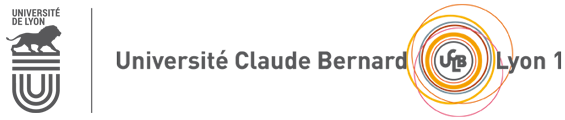
\includegraphics[width=0.5\textwidth]{figures/logo-lyon1.png}
  %  \end{center}
\maketitle

\keywords{Robotique développementale, affordance, clusterisation d'effets}

% \tableofcontents

\section*{Remerciements}
% \addcontentsline{toc}{chapter}{Acknowledgement}

Mon stage de 6 mois au sein de l'équipe AMAC à l'ISIR fût une formidable expérience. Je voudrai remercier Stéphane Doncieux, Alexandre Coninx et Carlos Maestre pour leur support et les nombreux conseils avisés qu'ils m'ont donnés.
Bénéficier de leur expérience et savoir a été un véritable atout pour mener à bien ce stage. Par ailleurs, ces 6 mois au sein de l'ISIR m'ont donné l'opportunité de découvrir davantage le monde de la recherche.

L'ISIR est l'un des meilleurs laboratoires de robotique en France et avoir la possibilité d'y faire un stage a été une extraordinaire opportunité de travailler dans un domaine passionnant et relativement jeune. D'autant plus que la robotique développementale et les robots auront un impact massif sur la vie des gens dans quelques décennies.

Reprendre des études en 2016 après avoir travaillé quelques années a été un véritable défi pour moi. En effet, cela supposait de quitter la ville où je vivais, de quitter mes amis et mon confort matériel ainsi que de revenir sur les bancs de l'université et de beaucoup travailler. J'allais avoir 30 ans et je me demandais si j'allais réussir dans ce Master 2.

% I am very glad to have the opportunity to pursue my works in PhD in the current months.

\section{Introduction}

% \epigraph{If I have seen further, it is by standing on the shoulders of giants.}{\textit{Isaac Newton}}

\subsection{Le laboratoire}

L'ISIR\footnote{http://www.isir.upmc.fr} (Institut des Systèmes Intelligents et de Robotique) est un laboratoire de recherche multi-disciplinaire créé en 2007 et co-tutellé par l'UPMC et le CNRS. Il rassemble des chercheurs de différents domaines : Sciences de l’Ingénieur et de l’Information ainsi que des Sciences du Vivant.

Les travaux de recherche à l'ISIR sont principalement centrés sur la modélisation et l'analyse des systèmes dynamiques artificiels et naturels, la conception optimale de systèmes robotiques interactifs, la commande des systèmes interactifs, la conception et le traitement du signal de systèmes perceptifs multimodaux, la modélisation des interactions homme - système, les modèles neuro-computationnels pour l’autonomie, l'apprentissage artificielle, l'adaptation bio-inspirée des systèmes et de leur commande. Dans cette perspective, le laboratoire est consitué de 4 équipes :
\begin{itemize}
\item AGATHE (Assistance aux Gestes et Applications THErapeutiques)
\item AMAC (Architectures et Modèles pour l'Adaptation et la Cognition)
\item INTERACTION
\item SYROCCO (SYstèmes RObotiques COmplexes)
\end{itemize}

J'ai réalisé mon stage de fin d'études au sein de l'équipe AMAC, encadré par Stéphane Doncieux. L'équipe est composée de 11 membres permanents et 13 membres non-permanents. Plusieurs membres sont spécialisés en neurosciences tandis que d'autres sont experts en robotique. Mon stage était orienté sur les affordances et a été financé par le projet DREAM\footnote{http://www.robotsthatdream.eu}. DREAM (Deferred Restructuring of Experience in Autonomous Machines) est is \textit{a robotics project that incorporates sleep and dream-like processes within cognitive architecture} et financé par le programme de recherche et d'innovation H2020 de l'Union Européenne.

Détails du projet Dream.

Une partie des membres de l'équipe AMAC travaille sur le projet DREAM (3 chercheurs, 2 post-doctorants, 3 doctorants et 4 stagiaires).
Seung Su, Léni et Jonathan : tracking d'objets et création de \textit{saliency map}.

Par exemple, plusieurs personnes travaillent sur la perception interactive. L'idée principale de la discipline est que pour segmenter des éléments (en l'occurrence des objects manipulables) dans une scène quelconque on ne peut pas se baser sur un a priori et pour compenser cela on va interagir avec l'environnement afin d'acquérir cette information. Le but d'un babillage est donc de produire une base de données. Une partie consiste à segmenter ce qui bouge et une autre doit pouvoir segmenter chaque objet. La segmentation de Leni me permet d'initialiser des hypothèses d'objets (ensemble de supervoxels) avec lesquels le robot interagis afin de valider ou non l'appartenance des supervoxels à un unique objet. La base de données qui est construite contient pour chaque objet les exemples de supervoxels qui lui ont été attribué.

Carlos : Apprentissage d'affordance
Pierre : reconnaissance de formes ?

Au terme de ce projet, les différents travaux de recherche des différents membres ont vocation à s'imbriquer les uns avec les autres dans le but de fournir un système global, allant de la détection et le suivi d'objet, à l'apprentissage d'affordances en passant par l'apprentissage de lancers de balle.

La Coruna : travaux sur les motivations extrinsèques.

\subsection{Environnement}

L'environnement de travail durant notre stage a consisté en différents modules reliés entre eux : ROS,  le simulateur  Gazebo, le framework Moveit et le robot Baxter. ROS is \textit{a flexible framework for writing robot software. It is a collection of tools, libraries, and conventions that aim to simplify the task of creating complex and robust robot behavior across a wide variety of robotic platforms\footnote{http://www.ros.org/about-ros/}}.

Gazebo est un simulateur\footnote{http://gazebosim.org}. La figure \ref{fig7} donne un aperçu d'une simulation lancée avec Gazebo.

Moveit

Quant au robot Baxter\footnote{http://www.rethinkrobotics.com/baxter/tech-specs/} (voir figure \ref{fig:baxter}), c'est un robot développé par Rethink Robotic et utilisé à la fois à des fin industrielles et de recherche. Ce robot antropormorphique à 2 bras dispose de 2 fois 7 degrés de liberté et de multiples  senseurs\footnote{http://sdk.rethinkrobotics.com/wiki/Hardware\_Specifications}.

\begin{figure}
	\centering
	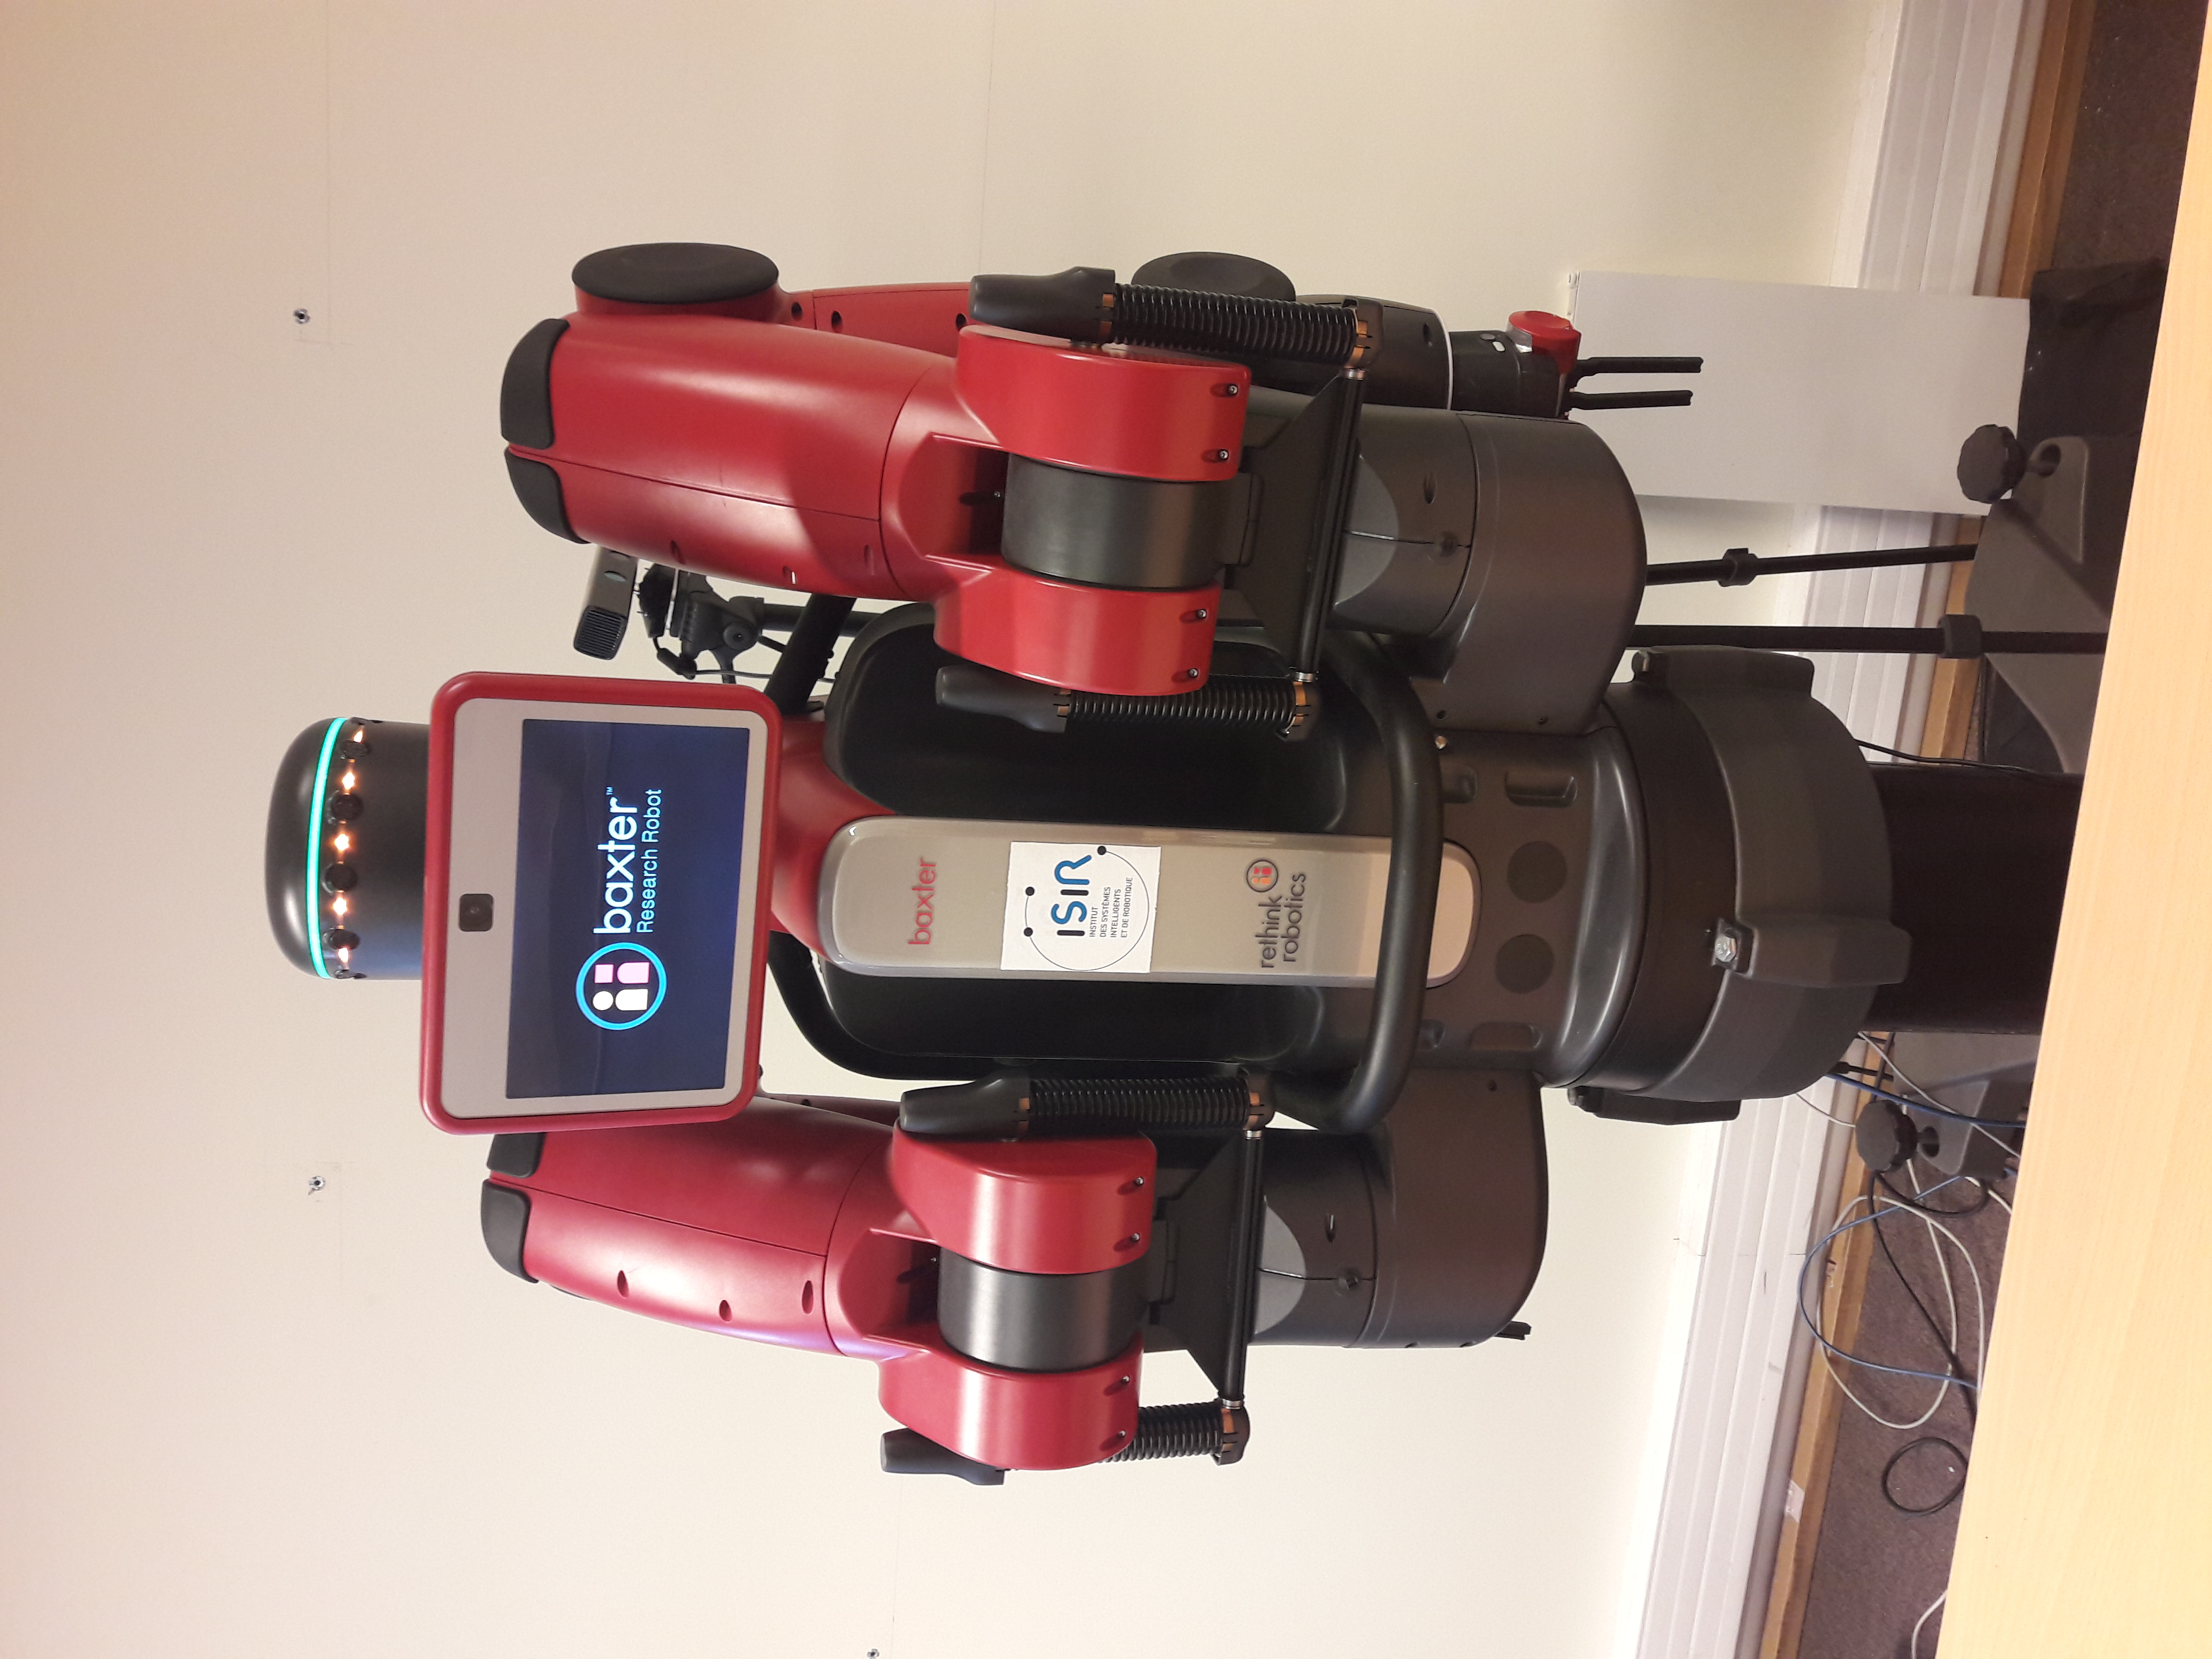
\includegraphics[angle=-90,width=.5\textwidth]{figures/baxter}
	\label{fig:baxter}
	\caption{Baxter robot}
\end{figure}

% \begin{figure}
% 	\centering
% 	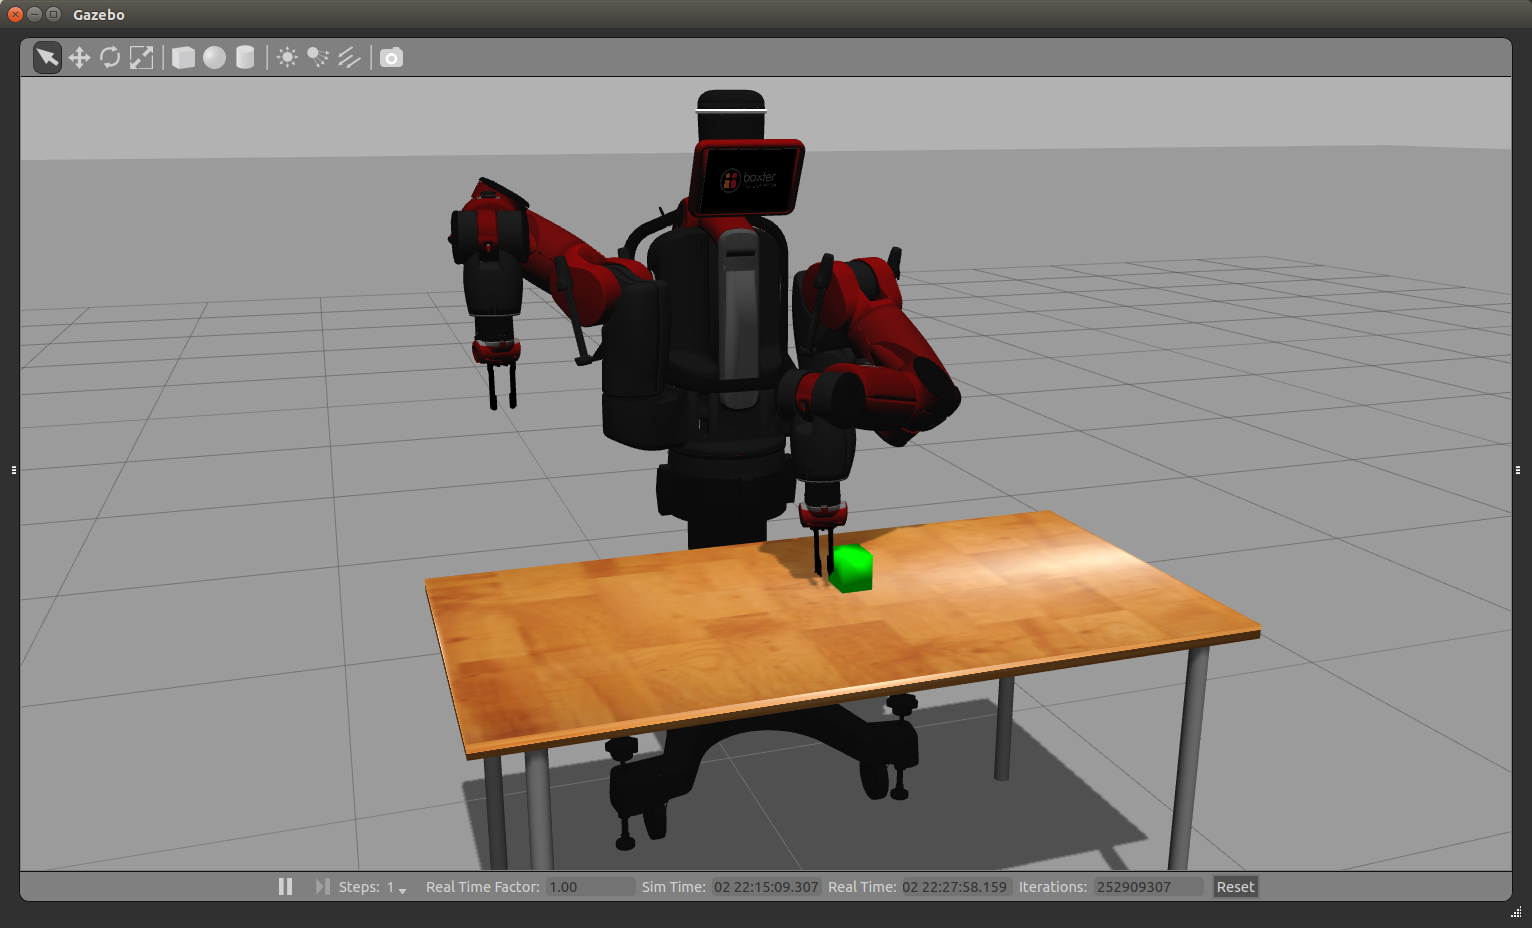
\includegraphics[width=\textwidth]{figures/gazebo}
% 	\label{fig:gazebo}
% 	\caption{Gazebo simulator}
% \end{figure}

\subsection{\'Etat de l'art}

Medias are nowadays talking about smart robots for tomorrow or the day after tomorrow. Such mass medias are explaining that people would find in their house, in a very near future,  a robot able to cook for you when you are short in time, mow the lawn and take care of elder people. However the path which conducts to these intelligent machines is still long and strewn with pitfalls. Several challenges have to be adressed before people interact with those robots as they do with other human people. Among these challenges, it is possible to cite movements learning.

% Developmental robotics

La robotique développementale est un domaine de recherche relativement jeune. Il dérive principalement de la robotique mais tire également ses racines des neurosciences cognitives.
Apprentissage autonome, généralisation
Plus efficace de créer un robot qui apprend qu'un robot auquel on apprend beaucoup de choses.

%% Affordances
% Affordances are an important concept when talking about sensorimotor learning. The term was defined in \cite{opac-b1085639} as what \textit{it offers the animal, what it provides or furnishes}. The main idea behing that term is to be able to discover the different actions that can be performed on an object, by considering available abilities. That definition establishes a strong relation between objects, actions and effects (see Figure \ref{fig:affordances}). For instance, for a robot with a grasper, affordances on a simple box are: pushing, grasping or touching. Furthermore, affordances can be also used to identify or reproduce action as described in \cite{4399517}.
% Affordances are objective, real and physical.
\subsubsection{Affordances}
L'apprentissage des affordances est une étape cruciale dans l'approche de la robotique développementale. Le terme a été défini dans \cite{opac-b1085639} comme \textit{it offers the animal, what it provides or furnishes}. L'idée principale derrière ce terme est d'être capable de découvrir les différentes actions qui peuvent être réalisées sur un objet, en considérant les capacités disponibles. Cette définition établit une relation forte entre les objets, les actions et les effets (see Figure \ref{fig:affordances}). Les affordances permettent de découvrir les différentes actions qui peuvent être réalisées sur un objet en fonction des capacités de l'acteur. Par exemple, pour un robot avec des pinces, une boîte offre les affordances  \textit{movable} et \textit{levable}, parmi d'autres. Les affordances sont capitables pour réaliser des actions, c'est-à-dire que le robot peut utiliser sa connaissance des affordances pour choisir la prochaine action à effectuer sur un objet pour accomplir une tâche. Par ailleurs, les affordances peuvent également être utilisées pour identifier ou reproduire des actions, telles qu'expliqué dans \cite{4399517}.

 %
 % A babbling approach consisting in applying random action and observing the corresponding effects can provide the data required to learn it, but where to start from? Defining a priori a limited set of possible actions and corresponding effects is a strong limitation to what the robot can achieve, but applying completely random actions results in a large set of possible effects that may be hard to exploit, in particular if the affordance is represented with a Bayesian network \cite{}.

\begin{figure}
	\centering
	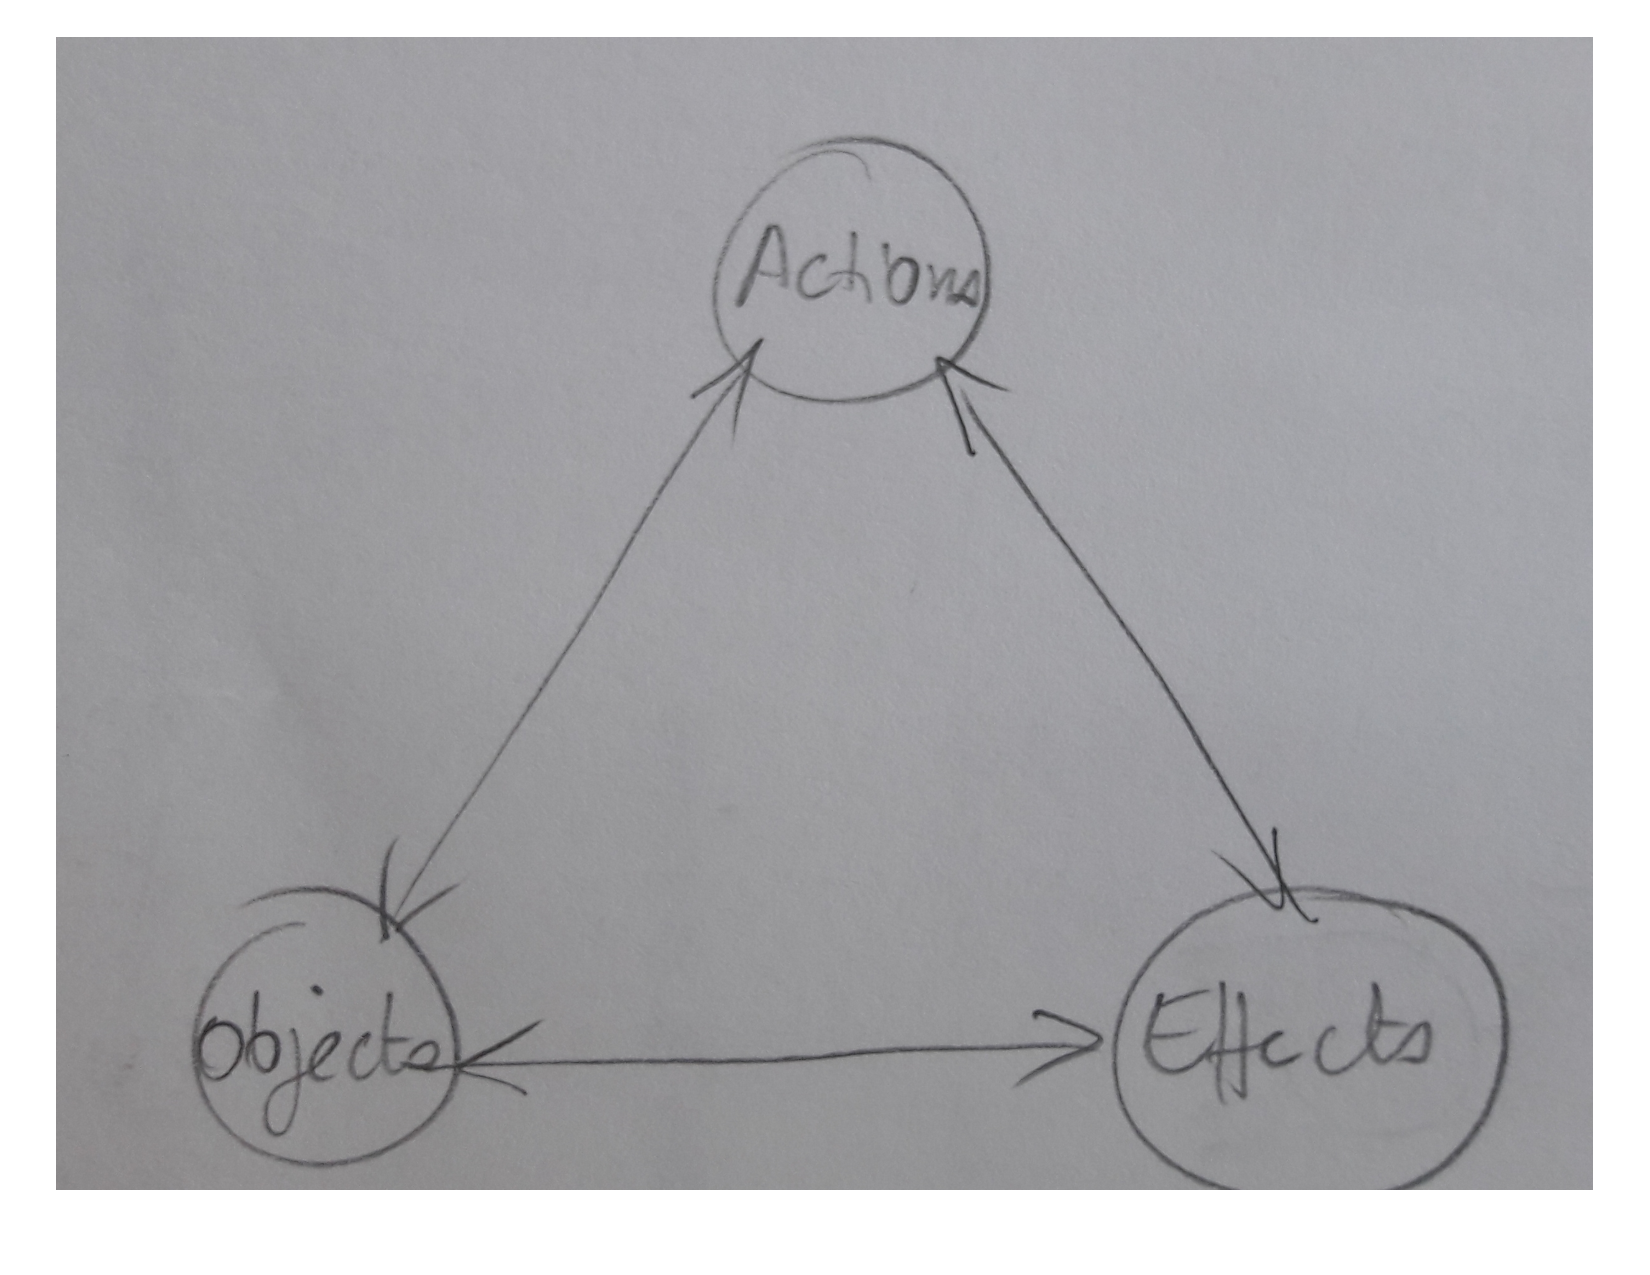
\includegraphics[width=.4\textwidth]{figures/affordances}
	\label{fig:affordances}
	\caption{Relationship between Actions, Ojects and Effects. \textit{To draw}}
\end{figure}

%% Boostrapping
\subsubsection{Boostrapping}
Meltzoff et al. explained in \cite{EDP:EDP157} that infants do not know a priori what muscle movements achieve a particular state of organ relations. The authors call that process body babbling, directly inspired from babbling when infants experiment vocal sounds. In short, they explain that infants do repeated moves as a game. Eventually, after a certain amount of time and repetitions, infants would learn the relation between the moves they perform and theirs effects. That concept was reused in developmental robotics. Indeed, for a robot, learning affordances requires to interact with the environment throught an exploration stage, which corresponds to babbling. Several heuristics exist to perform that exploration.

%% Motor babbling
\subsubsection{Motor babbling}
Une première approche naïve consiste à utiliser des mouvements aléatoires. Cette approche est la plus simple à implémenter mais elle peut générer un nombre important de mouvements qui ne produisent pas de contact avec les objets.

Another approach is presented in \cite{Maestre2015} where Maestre et al. described the use of Novelty Search, an evolutionary algorithm, in order to generate trajectories aimed at maximizing the environment's exploration. Results show that trajectories allowing to touch objects are more and more privilegied over the different generations.

%% Intrinsic motivations
\subsubsection{Intrinsic motivations}
Une troisième approche réside dans les motivations intrinsèques. Ce concept a été décrit par Ryan et Deci, puis par Hull et plus tard formalisé en modèles computationnels par Oudeyer et Kaplan dans \cite{10.3389/neuro.12.006.2007}. Les motivations intrinsèques permettent d'explorer progressivement l'environnement en favorisant une spécialisation progressive des <modules>. Ce concept est utilisé en robotique et spécifiquement en robotique développementale.

% A third approache resides in intrinsic motivations, a concept described by Ryan and Deci, then by Hull and later formalized in computational models by Oudeyer and Kaplan \cite{10.3389/neuro.12.006.2007}. Intrinsic motivations allow to explore the environment by progressively specializing. Concept reused in robotics and especially in developmental robotics.

Context: The ability to perform in an open-ended environment and to build on previously acquired knowledge to quickly adapt to changes and unknown situations is key to building
multi-purpose assistive robots which can be helpful in a wide range of realistic situations.

%% Cognitive Developmental
Cognitive Developmental robotics is a promising approach to create robots with higher cognitive functions as shown in \cite{Asada2009} by Asada et al.

%% Use of tools
\subsubsection{Utilisation d'outils}
Au delà des affordances, des recherches prometteuses se concentrent sur la manipulation d'outils. Dans \cite{Goncalves2014}, Gonçalves et al. proposent une approche intéressante pour apprendre les afforfances visuelles d'objets ou d'outils. Dans cet article, un robot apprend les caractéristique visuelles d'objets et d'outils à l'aide de descripteurs visuels. De de façon, ils montrent que le robot est capable de réaliser une action spécifique ou d'obtenir un résultat désiré. L'utilisation des descripteurs visuels permet au robot de généraliser avec des objets inconnus.

% Beyond affordances, promising researches focused on tool usage. In \cite{Goncalves2014}, Gonçalves et al. proposed an interesting approach to learn visual affordances of objects and tools. In that paper, a robot learned visual features of objects and tools by using visual descriptors. Then, they show that the robot is able to perform a specific action or obtain a desired result. The use of visual descriptors allow the robot to generalize with unknown objects.

%% Bayesian network
Once sensorimotor babbling has been performed, the relationships between objects, actions and effects need to be modeled. Bayesian networks are a method to achieve that. They are probabilistic model that represent the relationship between their variables. In \cite{4456755}, Montesano \textit{et al} presented a Bayesian betwork model for learning object affordances.

Our work focused on improving the paper of \cite{Ugur2011}. In that paper, Ugur \textit{et al}.
described a system that allows a robot to learn goal emulation by using learnt affordances. In order to that, the robot follows an observation stage then an imitation stage.

- bootstrap object-oriented behavior
- discover object in an unknown environment

\subsection{Related work}

Ce stage de fin d'études l'a été dans le cadre du projet DREAM, débuté en 2015. Ce projet implique 5 partenaires académiques: UMPC/CNRS (coordinateur), ENSTA ParisTech, Universidade da Coruña, Vrije Universiteit Amsterdam et Queen Mary University of London. Ces différents acteurs ont différents rôles au sein du projet DREAM. See waves.

% \`A l'issue du projet DREAM, les différents modules
At the end of the DREAM project, the different modules are aimed at be linked together.

Our work is directly based on actual PhD student's work on learning affordances inspired from motor babbling.

% Linkedin: "The main goal of this thesis is the autonomous creation by a robot of a minimal directory of concepts related to its morphology, its environment, and the accomplished tasks executed. The robot must be able to build and update its internal world model through interactions with its environment (cognitive bootstrapping). This work follows the approach proposed in developmental robotics, inspired by the development of the infants, where abstract concepts are created progressively based on the sensori-motor capabilities of an agent.

% Executed in an iterative loop, a dataset is created by the robot through the babbling of its environment; some candidate world models are defined based on the data gathered; and a new dataset is created, in order to discriminate these models, improve them and generate new simpler ones."

\section{Notre travail}

% \epigraph{Artificial intelligence is the science of making machines do things that would require intelligence if done by men.}{\textit{Marvin Minsky}}

\subsection{Adaptative discretization}

\subsubsection{Previous works}

Afin de réaliser cela, le nombre des actions prédéfinies disponibles était fixé à 4 (\textbf{Gauche}, \textbf{Droite}, \textbf{Haut}, \textbf{Bas}). Voir figure~\ref{fig:trajectories}.

\begin{figure}
	\centering
	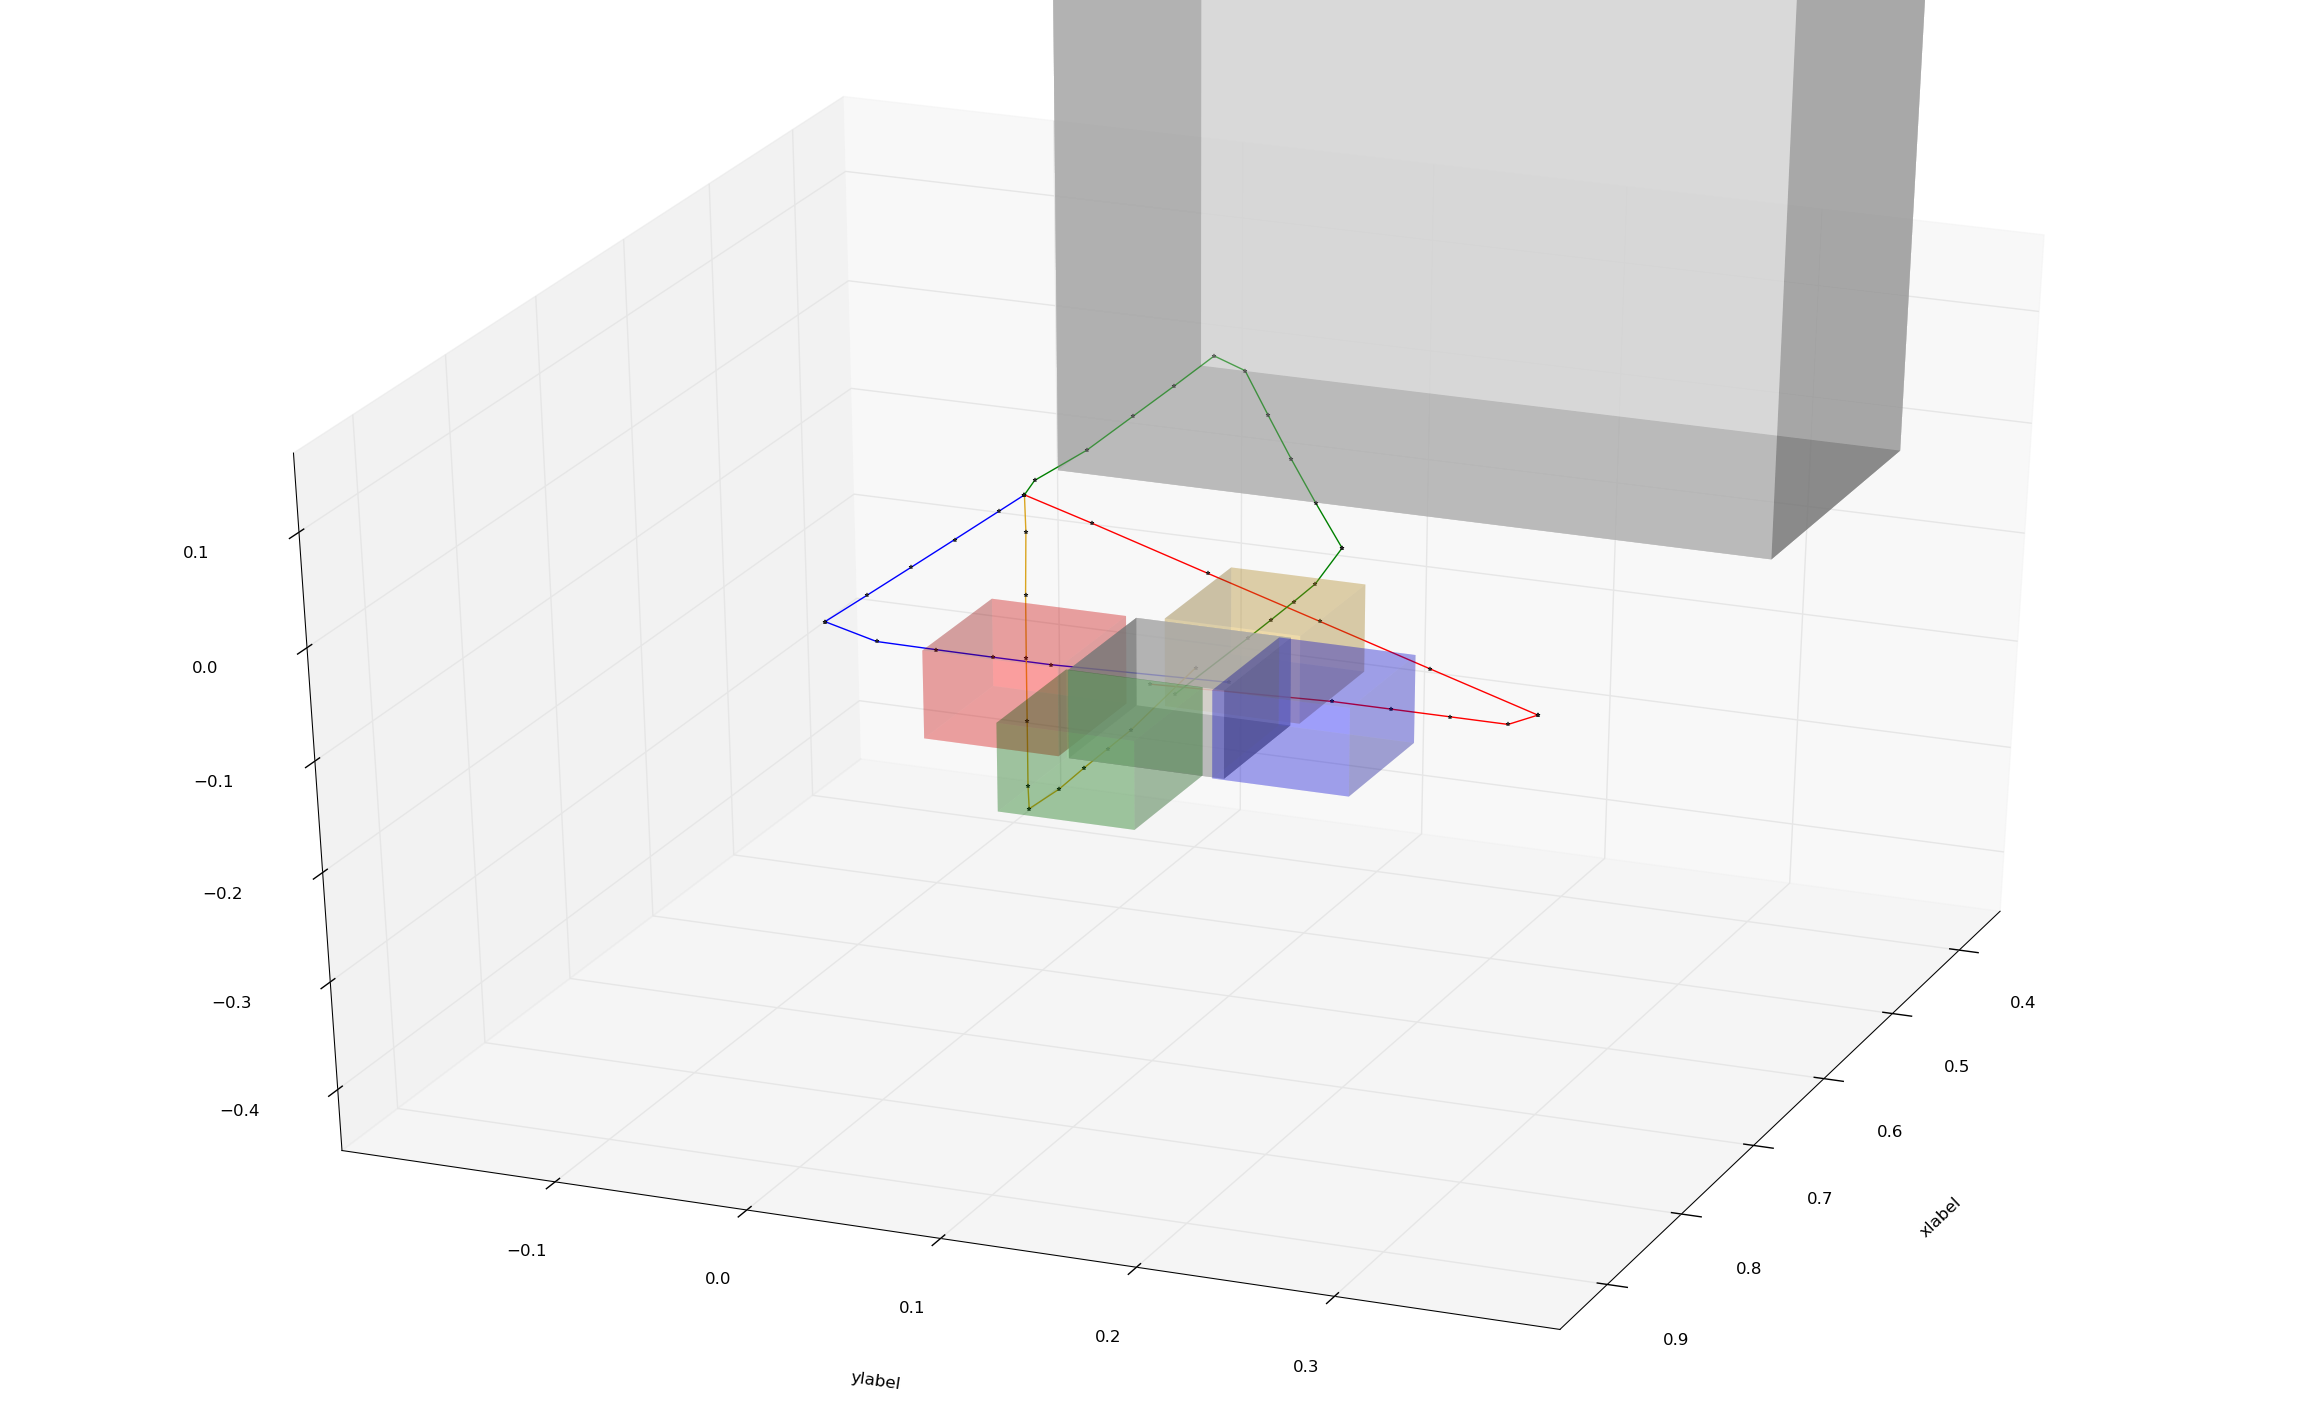
\includegraphics[width=\textwidth]{figures/trajectories}
	\caption{Movements trajectories performed by the robot (gray shape in background). Initial position of the object is represended by the gray cube in the center. Each colored cube corresponds to a movement of the same color (\textit{e.g.} the red cube is the final position of the gray cube after being pushed by the the robot's end effector along the red trajectory).}
	\label{fig:trajectories}
\end{figure}

En raison de la nécessesité de généraliser,
For purpose of generalization, it would not be possible to let such a value. The first step of the internship focused on the goal of achieving environment's \textbf{adaptative discretization}. The main idea behind is to let the agent itself discover actions without specifying an arbitraty number of actions to discover.  In order to do so, clusterization is used to distinguish those different actions. X-means algorithm\cite{Pelleg:2000:XEK:645529.657808}, based on k-means, was used at the beginning. Basically, X-means is a k-means algorithm's generalization, which finds itself the best value for $k$.

% \begin{figure}
% 	\centering
% 	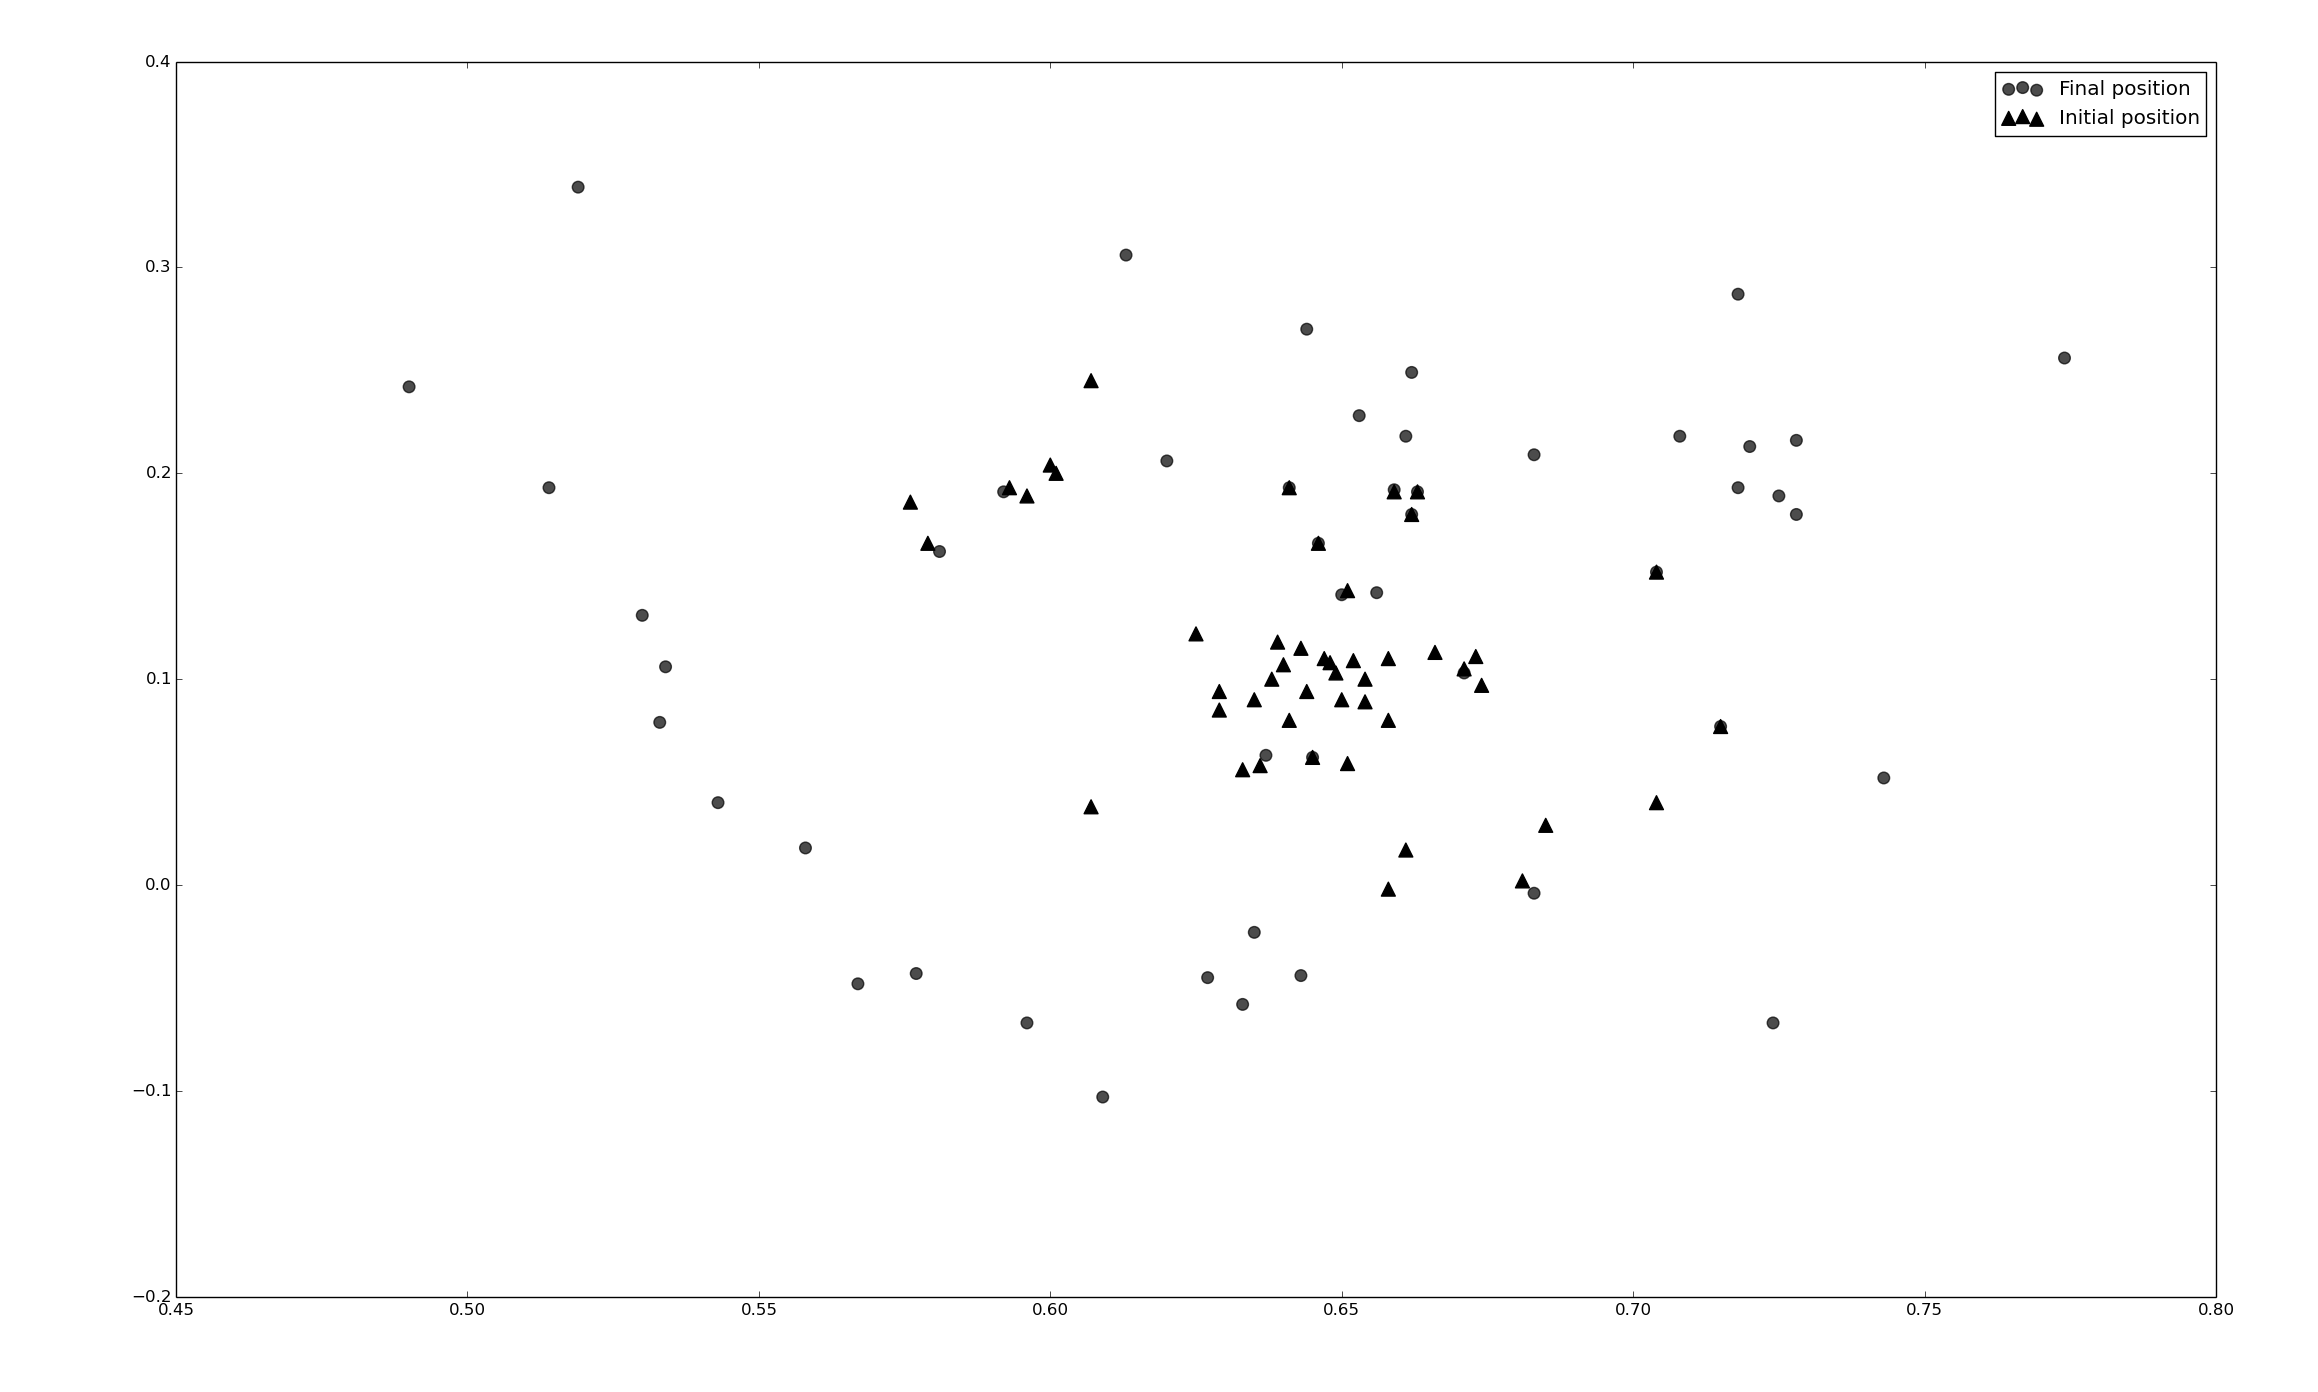
\includegraphics[width=\textwidth]{figures/before_offset_correction.png}
% 	\label{fig:plot_before}
% 	\caption{Original dataset}
% \end{figure}
%
% \begin{figure}
% 	\centering
% 	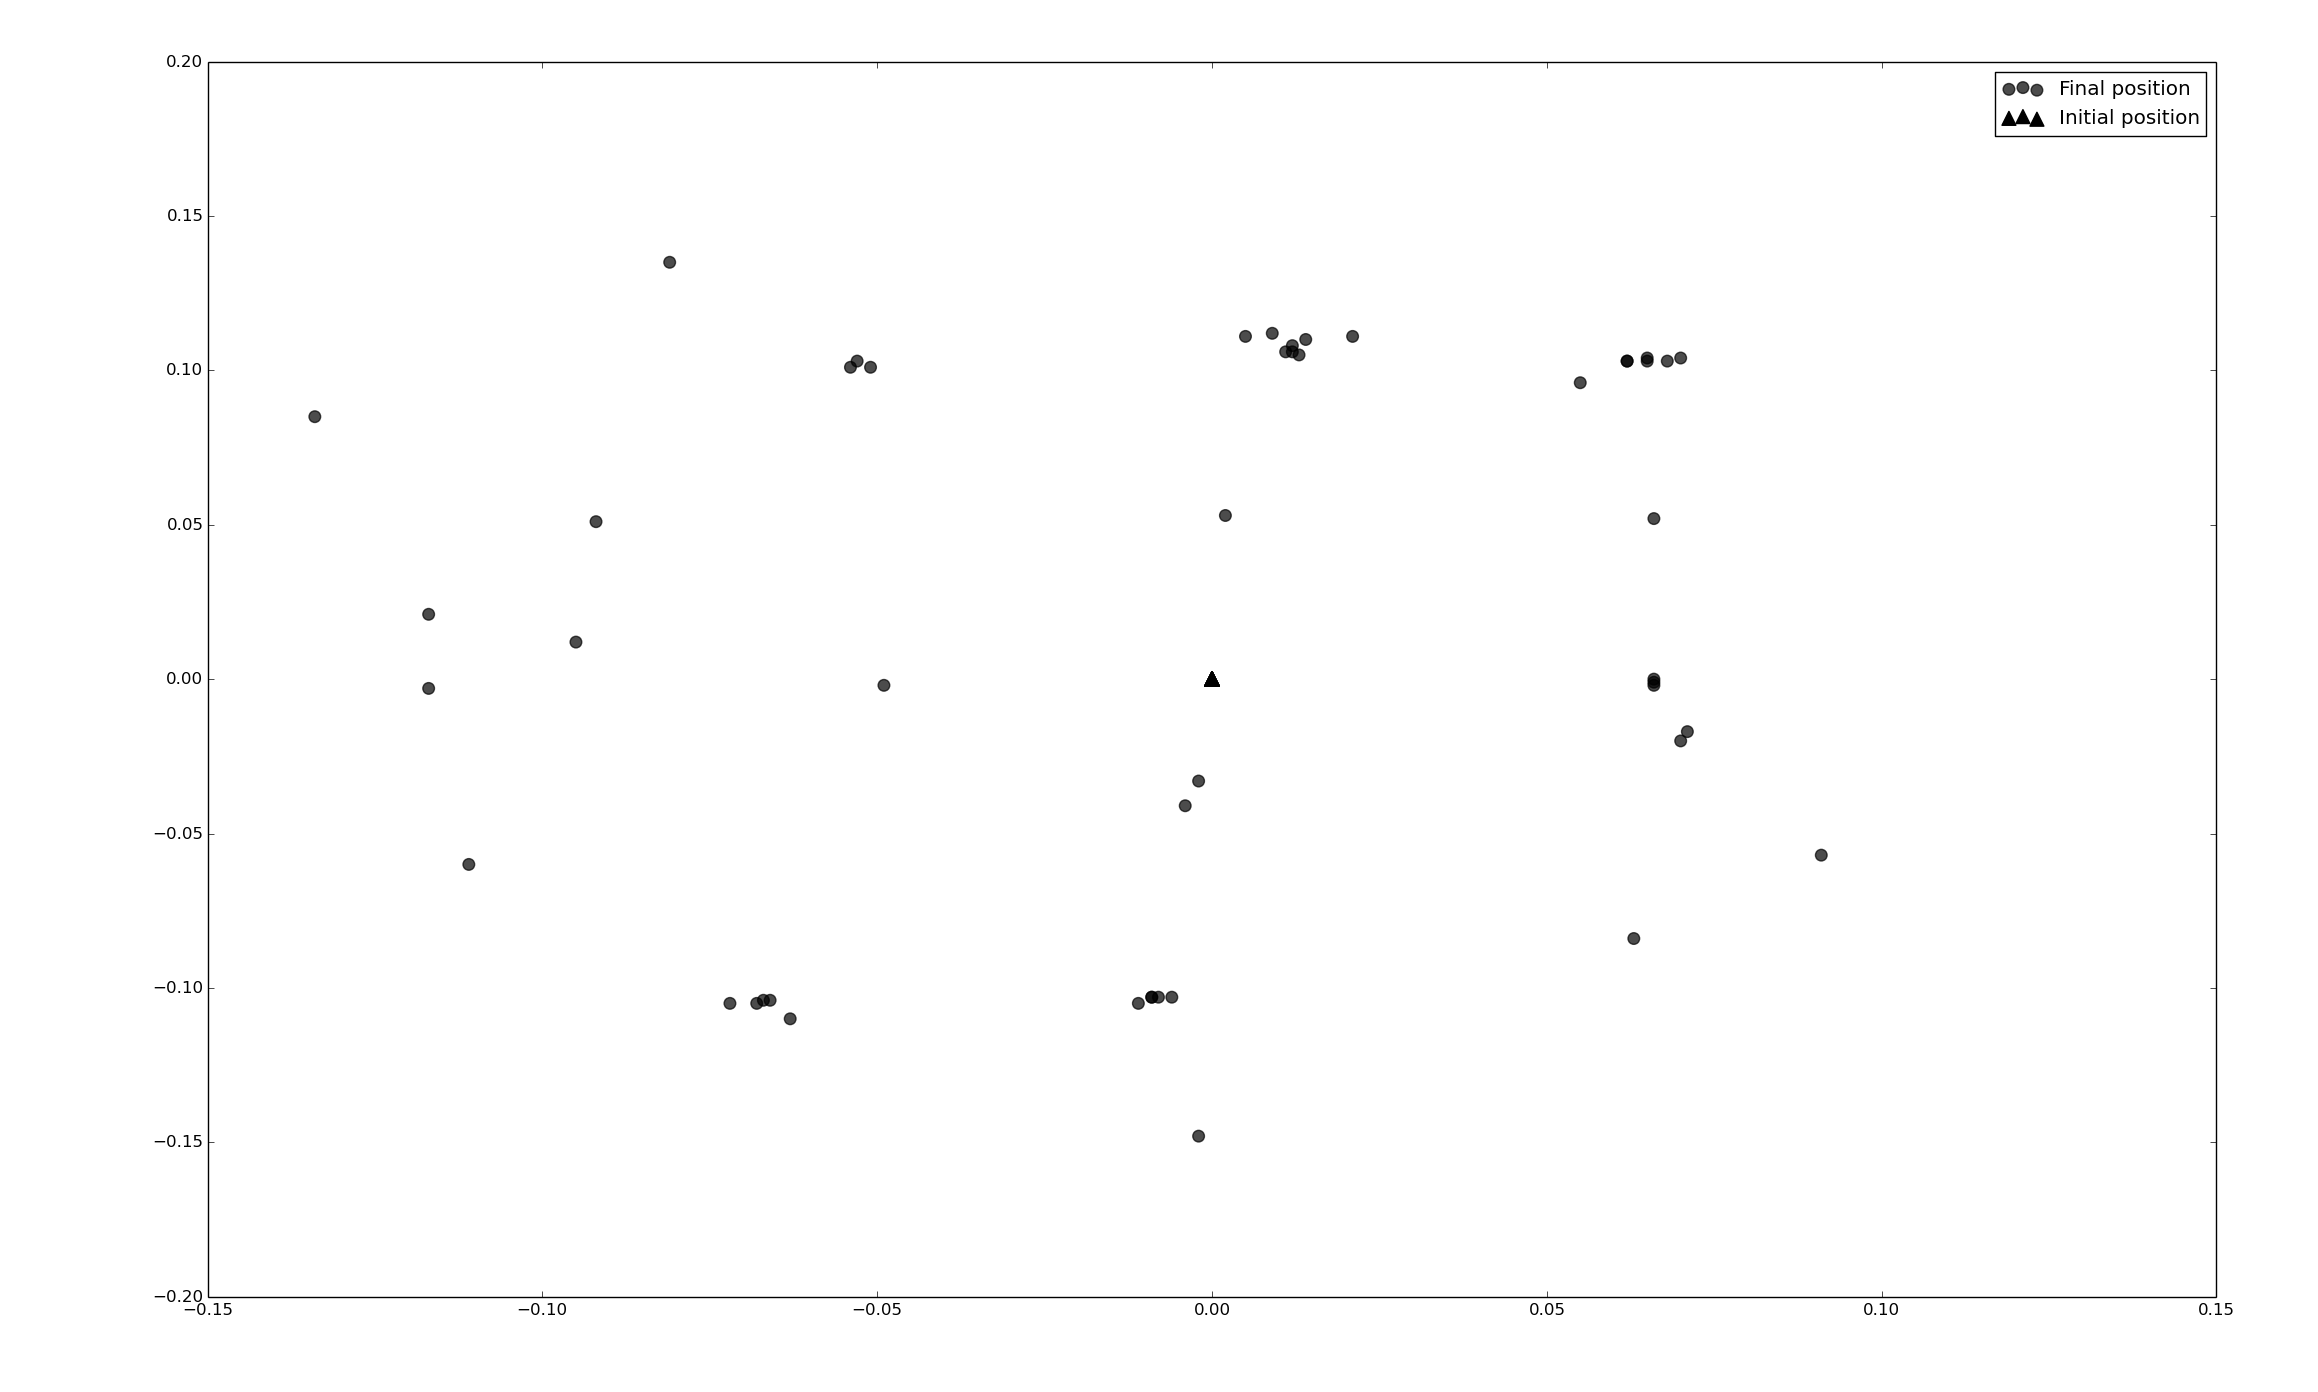
\includegraphics[width=\textwidth]{figures/after_offset_correction.png}
% 	\label{fig:plot_after}
% 	\caption{Trajectories where initial points' offset are corrected}
% \end{figure}

\subsubsection{Algorithmes de clustering}

En nous basant sur \cite{Xu2015}, \cite{Andreopoulos2009}, \cite{Fahad2014} et \cite{Sajana2016}, nous avons réalisé une synthèse des algorithmes de clustering les plus communément utilisés, groupés en catégories (c.f. Annexe pour plus de détails). Afin de filter et sélectionner les algorihtmes, nous avons choisi des critères non arbitraires. En se référant à la généralisation mentionnée ci-dessus, un premier critère concerne la nécessité de ne pas fournir le nombre attendu de clusters en paramètre. En effet, puisque le système doit être capable de trouver lui-même le nombre correct d'actions. Un second critère concerne la possibilité de travailler avec de nombreuses dimensions et un troisième concerne la disponibilité d'une implémentation en Python ou C++. Les algorithmes qui ne satisfaisaient pas à ces critères ont été rejetés.

7 algorithmes de clustering ont été comparés lors de cette première phase : X-means\textsuperscript{1}, Affinity Propagation\textsuperscript{1}, DBSCAN\textsuperscript{2}, HDBSCAN\textsuperscript{2}, OPTICS\textsuperscript{2}, Mean-Shift\textsuperscript{2} et Level Set Tree. (1) correspondent à des algorithmes de partitionnement et (2) correspondent à des algorithmes basés sur la densité.

% Based on \cite{Xu2015}, \cite{Andreopoulos2009}, \cite{Fahad2014} and \cite{Sajana2016}, we reviewed the most common algorithms used for clustering, grouped in categories (see annex for details). Non-arbitrary criteria were required for filtering algorithms. According to the generalization mentioned above, a first criterion concerns the requirement to pass the number of clusters as input parameter. Indeed, as the system should be able to find itself the correct number of actions. A second criterion concern the possibility to work with high dimensionality and a third one is the implemenation's availabily in Python or C++. Algorithms that did not suit to those parameters were discarded.

% 7 implementations of clustering algorithm were compared: X-means\textsuperscript{1}, Affinity Propagation\textsuperscript{1}, DBSCAN\textsuperscript{2}, HDBSCAN\textsuperscript{2}, OPTICS\textsuperscript{2}, Mean-Shift\textsuperscript{2} and Level Set Tree. (1) are partitioning algorithms and (2) are density-based algorithms.

% Amongst those algorithms, Affinity Propagation is the only one which found a correct result according to the input dataset. It is able to detect the 7 different clusters without finding outliers. See Figure~\ref{fig:ap}.

The intuition behind that choice is based on the fact that the different categories of actions have roughly the same end position. In other terms, a \textbf{Left} action will end in the specific area for left actions. Hence, a large amount of space will be empty and will not contain any end positions. The points distribution would lead to focus on finding areas of high density. For that purpose, density-based algorithms exist.

Afin de comparer les différents algorithmes, une série de tests a été réalisée avec 2 jeux de données différents : un dataset avec une distribution uniforme de points et un jeu de données généré en simulation.


% \begin{figure}
% 	\centering
% 	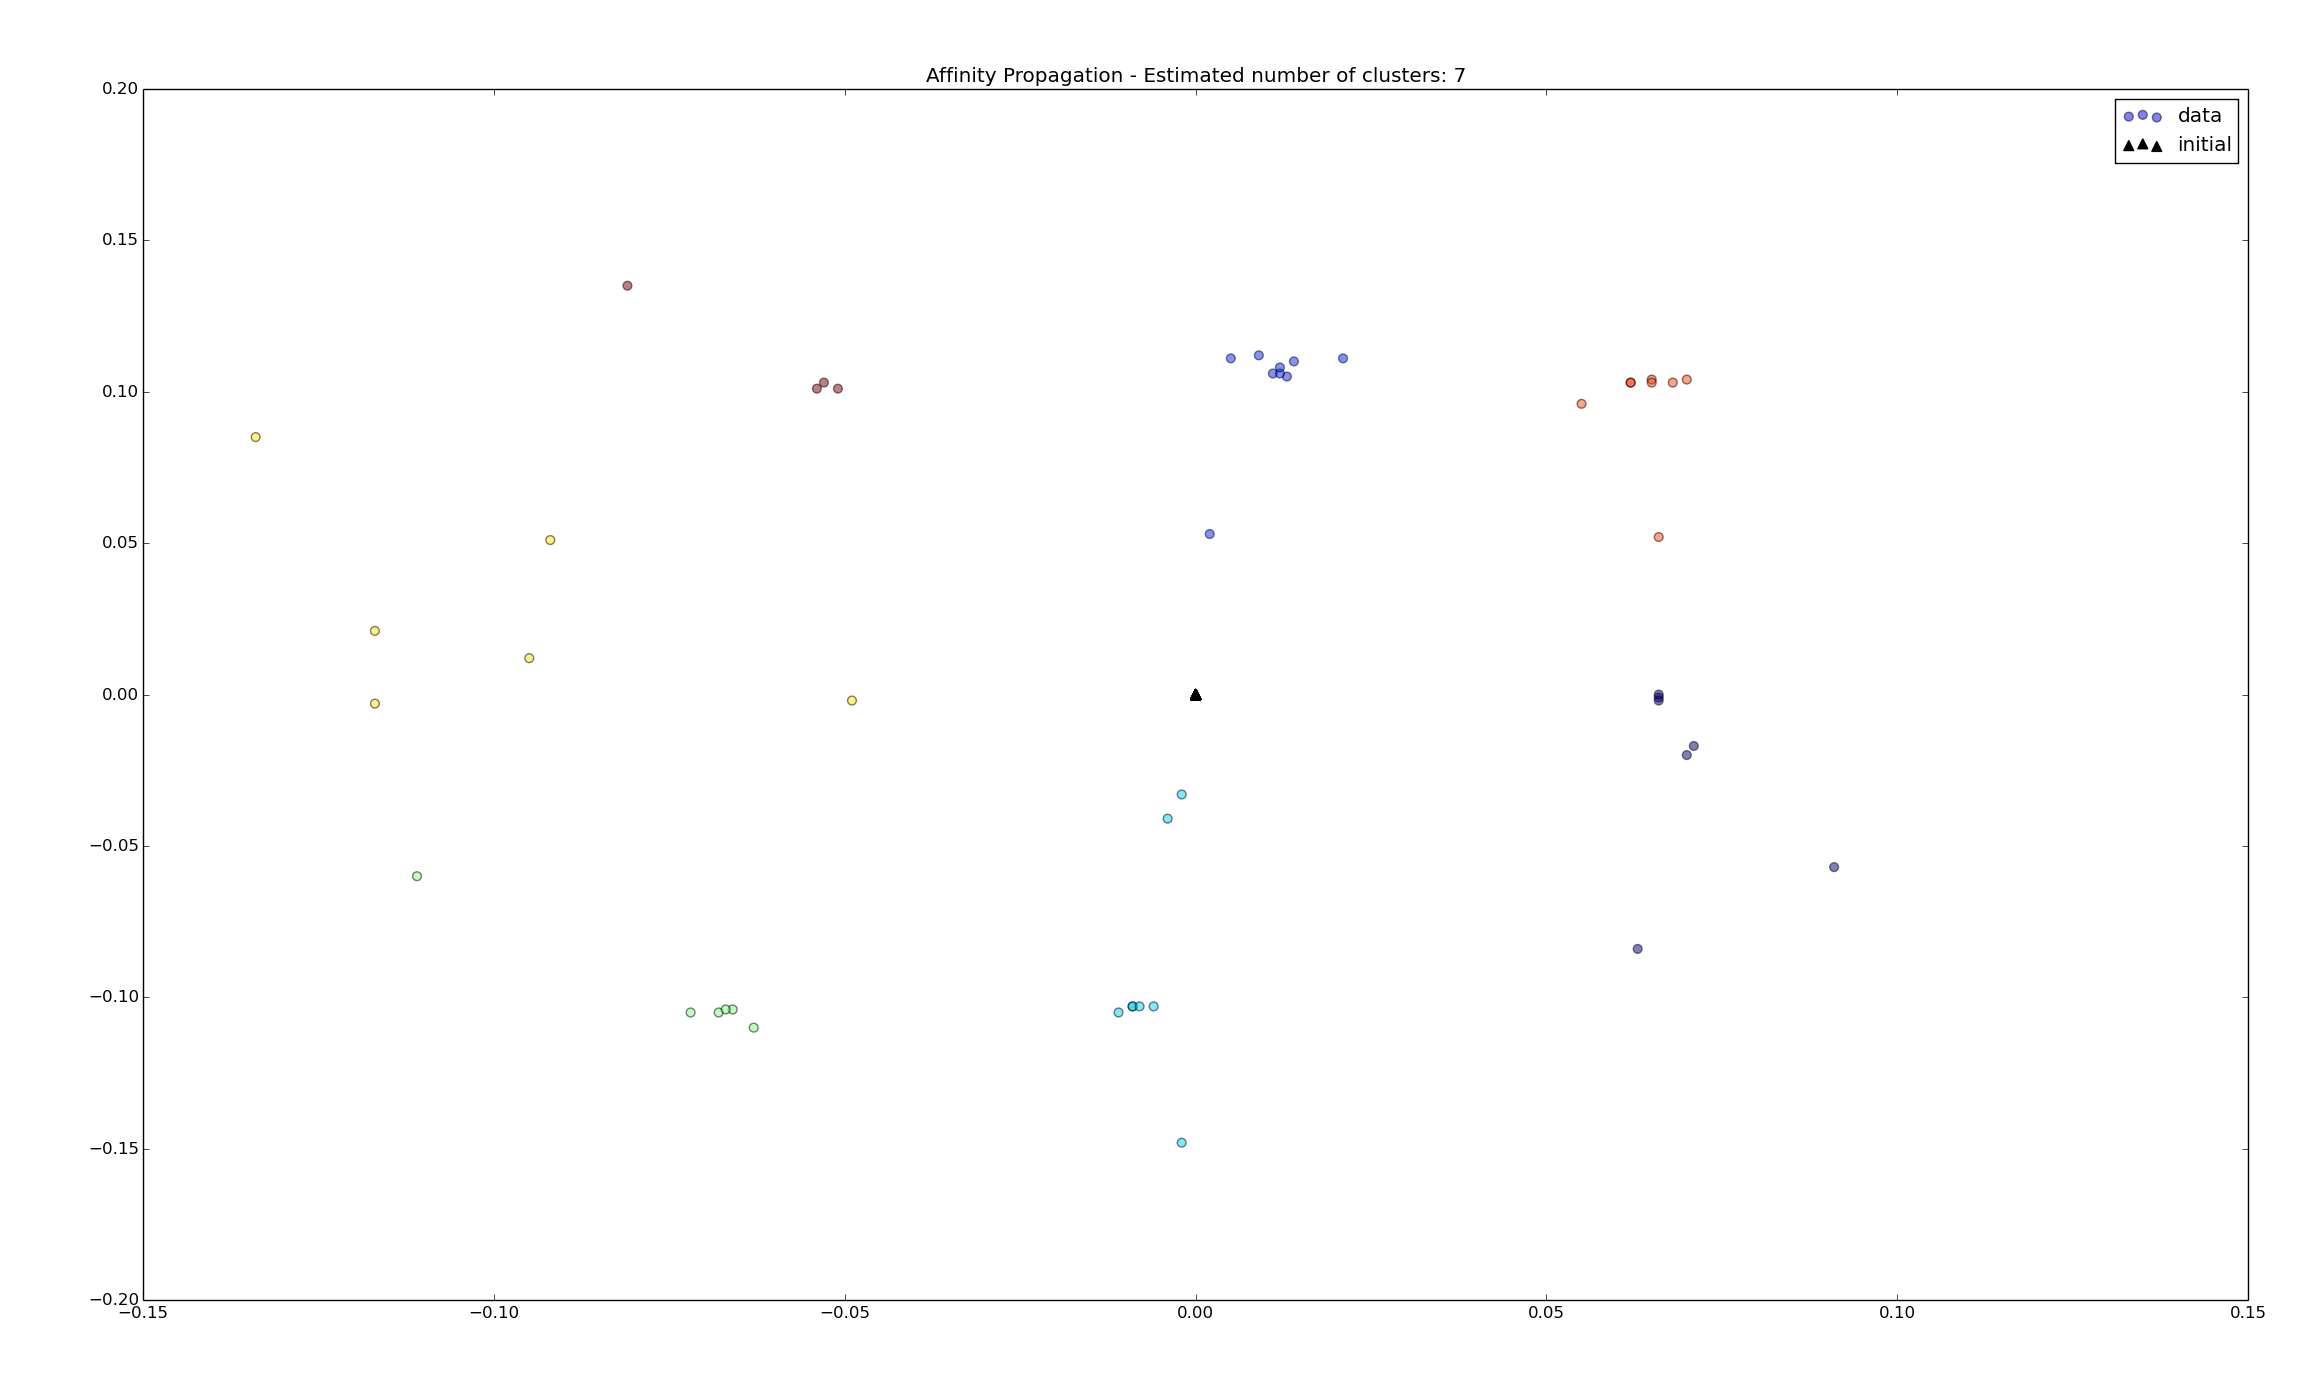
\includegraphics[width=\textwidth]{figures/clustering_results/AP}
% 	\caption{Clustering with Affinity Propagation. AP clusters correctly the dataset. Parameters are: \textit{damping=0.5, preference=-0.0095}}
% 	\label{fig:ap}
% \end{figure}

% Clustering results were very dependent on the dataset. For instance, in the Figure~\ref{fig:comparison}, the clusters are not perfect. Indeed, both clusters at bottom left (blue and yellow) should have been grouped into one cluster. That single cluster is, however, also difficult to predict for human.

% \begin{figure}
% 	\centering
% 	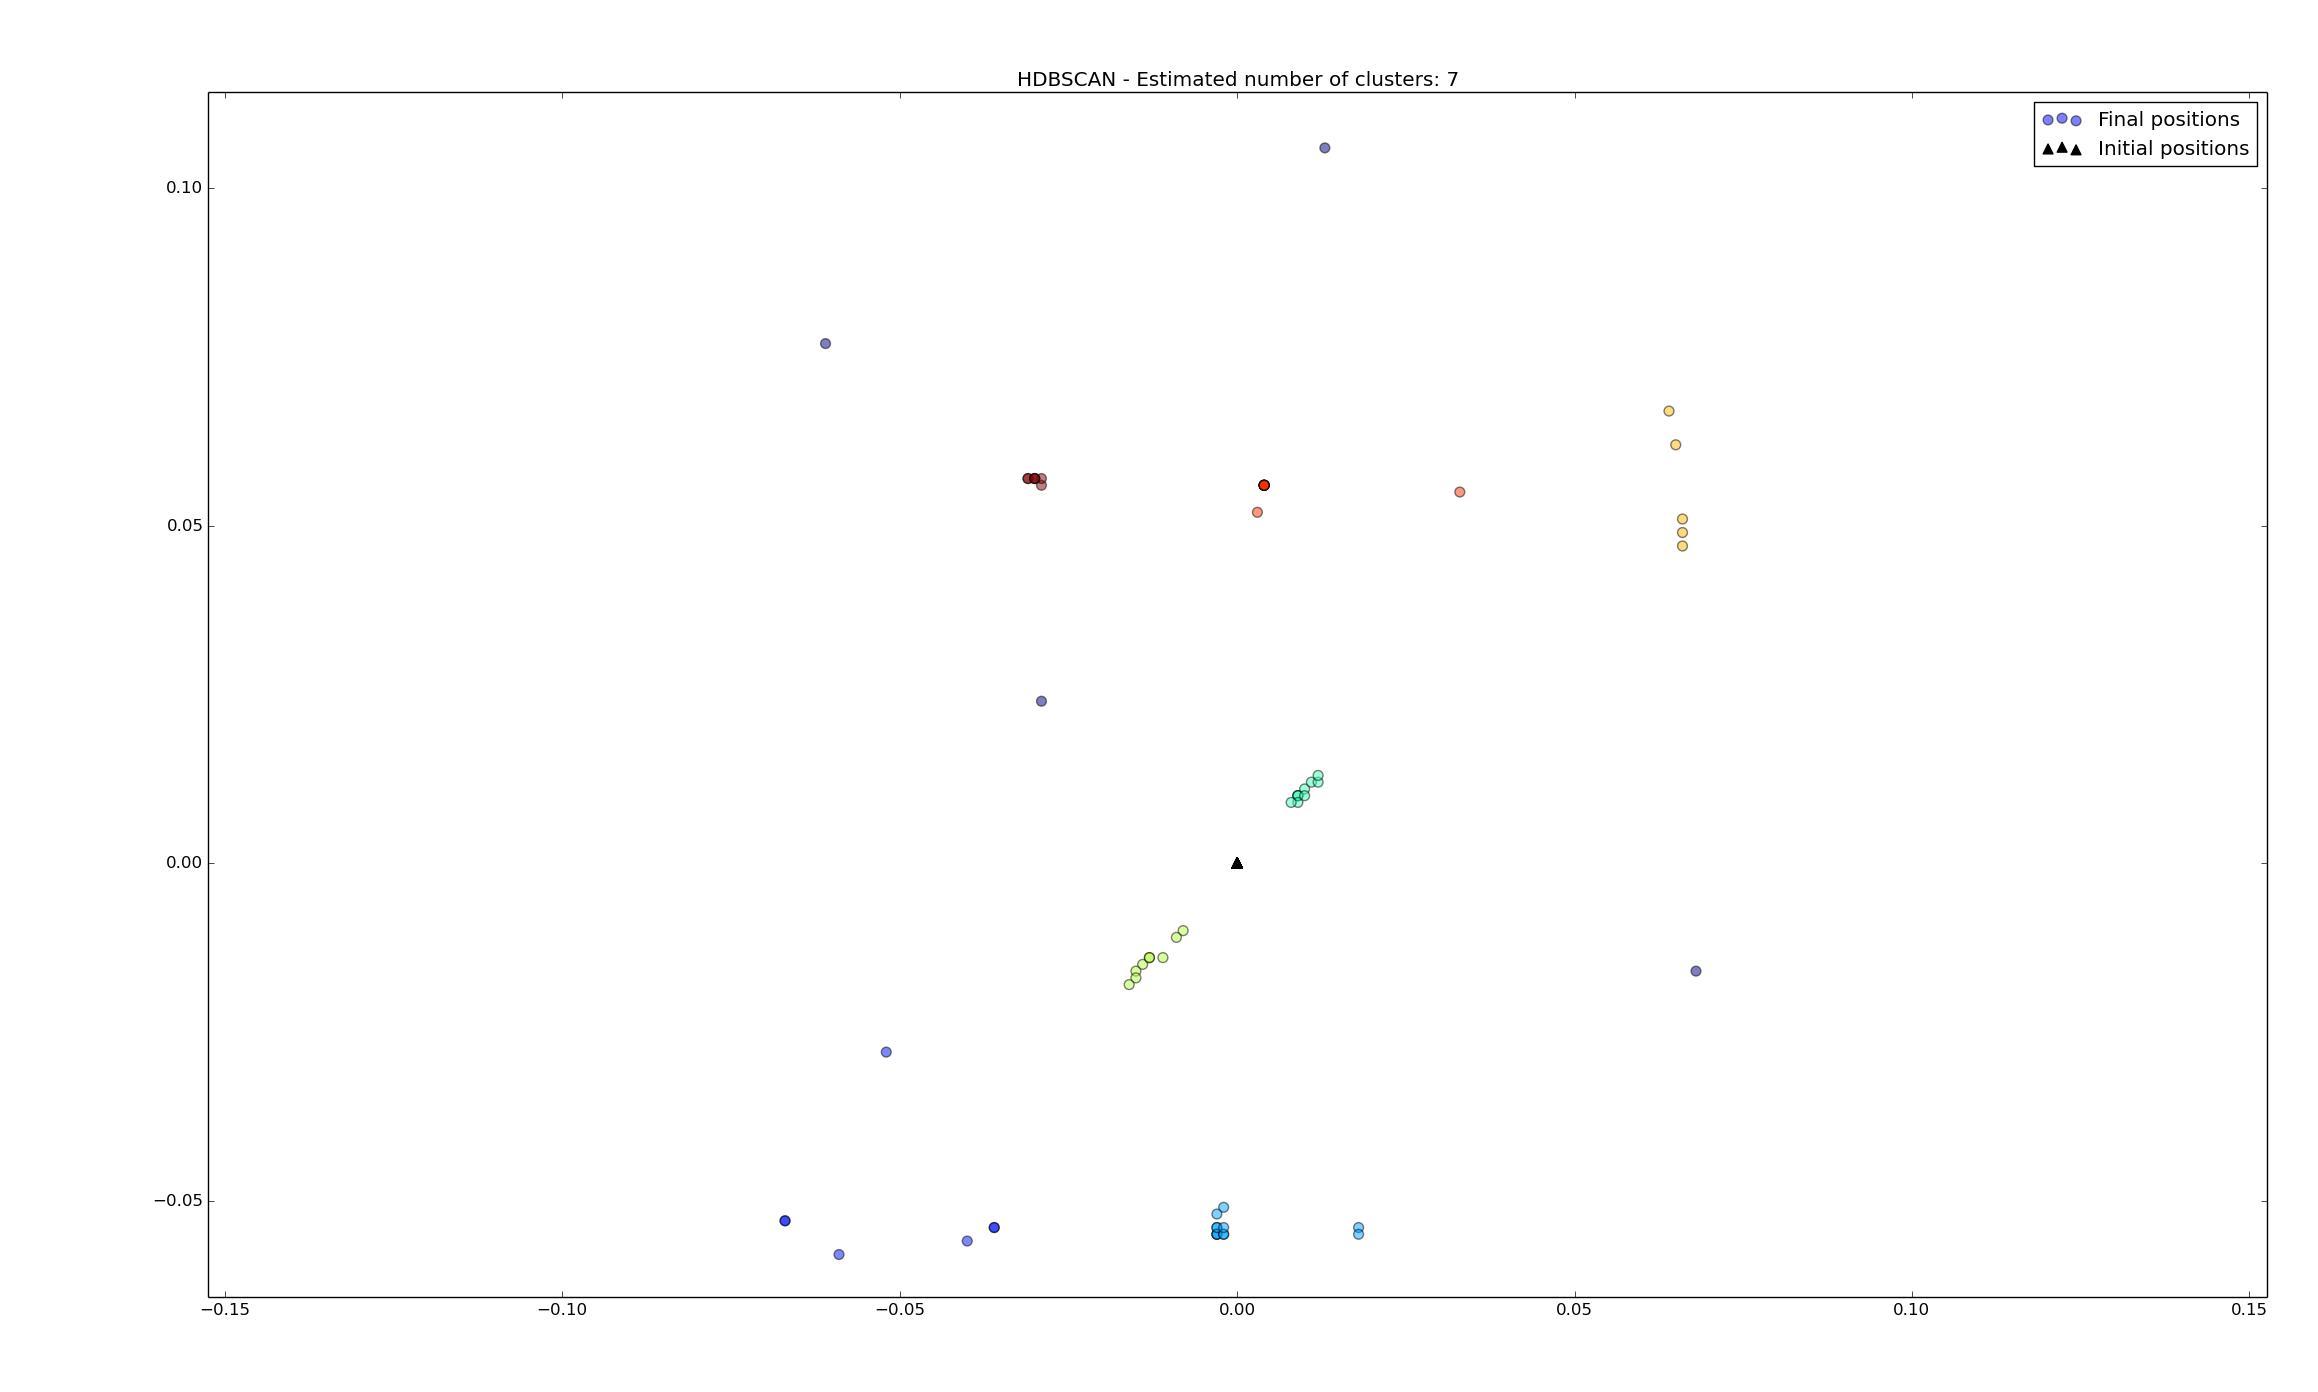
\includegraphics[width=\textwidth]{figures/ds4_non_normalized}
% 	\caption{}
% 	\label{fig:non_norm}
% \end{figure}
%
% \begin{figure}
% 	\centering
% 	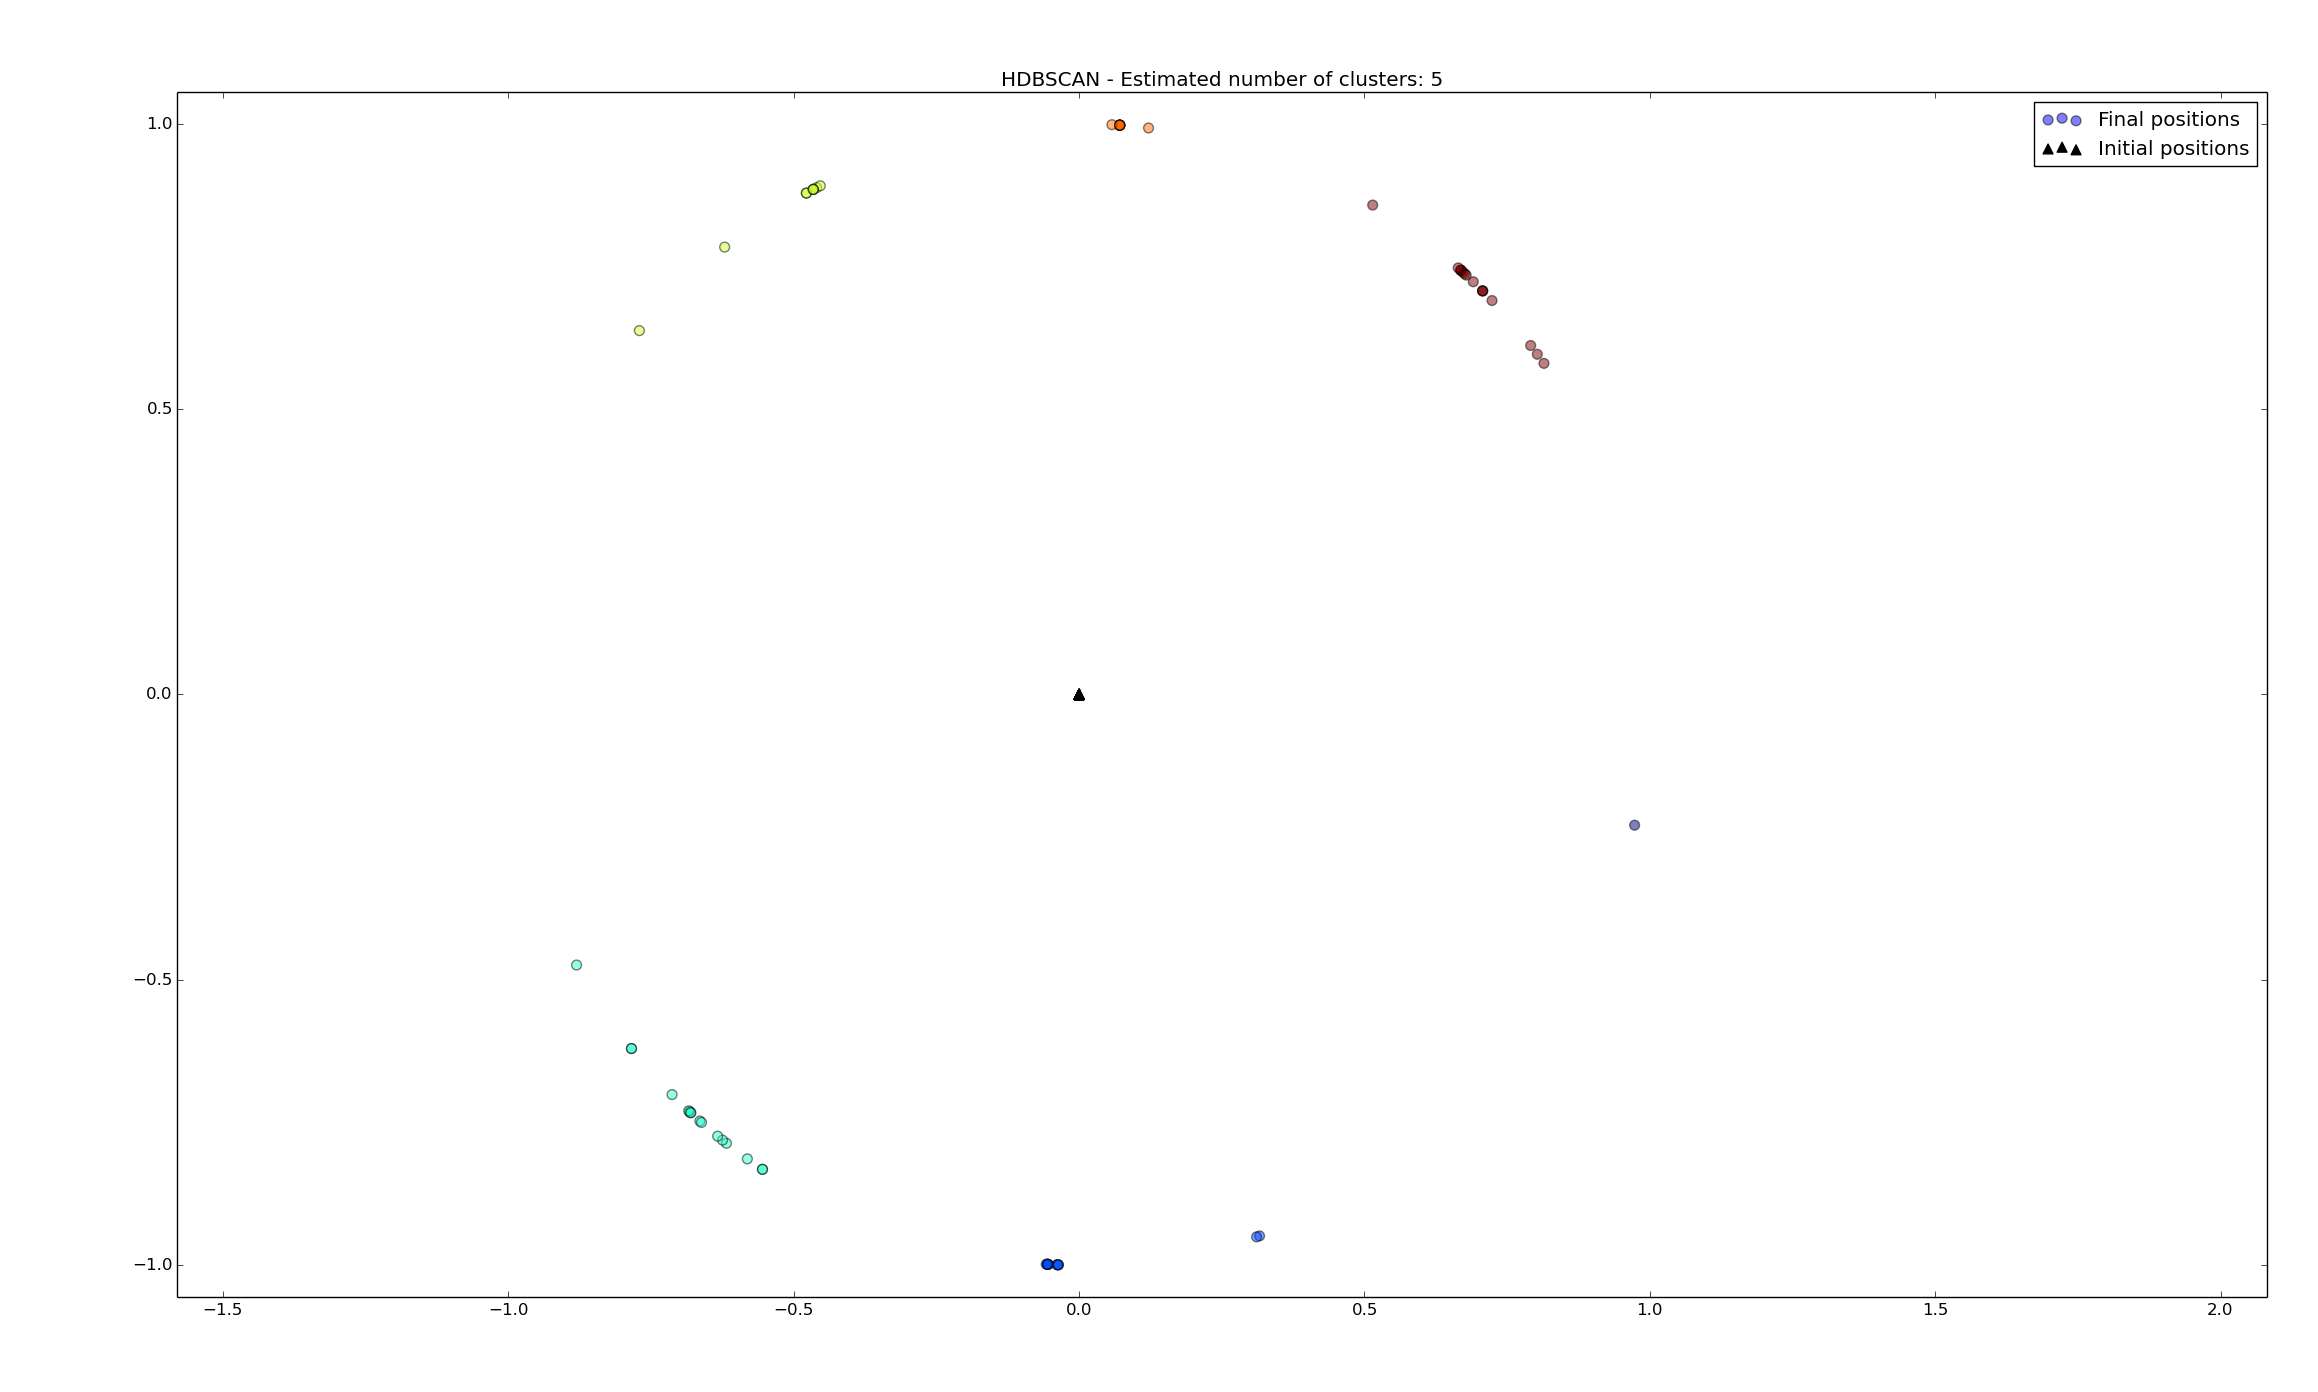
\includegraphics[width=\textwidth]{figures/ds4_normalized}
% 	\caption{}
% 	\label{fig:norm}
% \end{figure}

% \begin{figure}
% 	\centering
% 	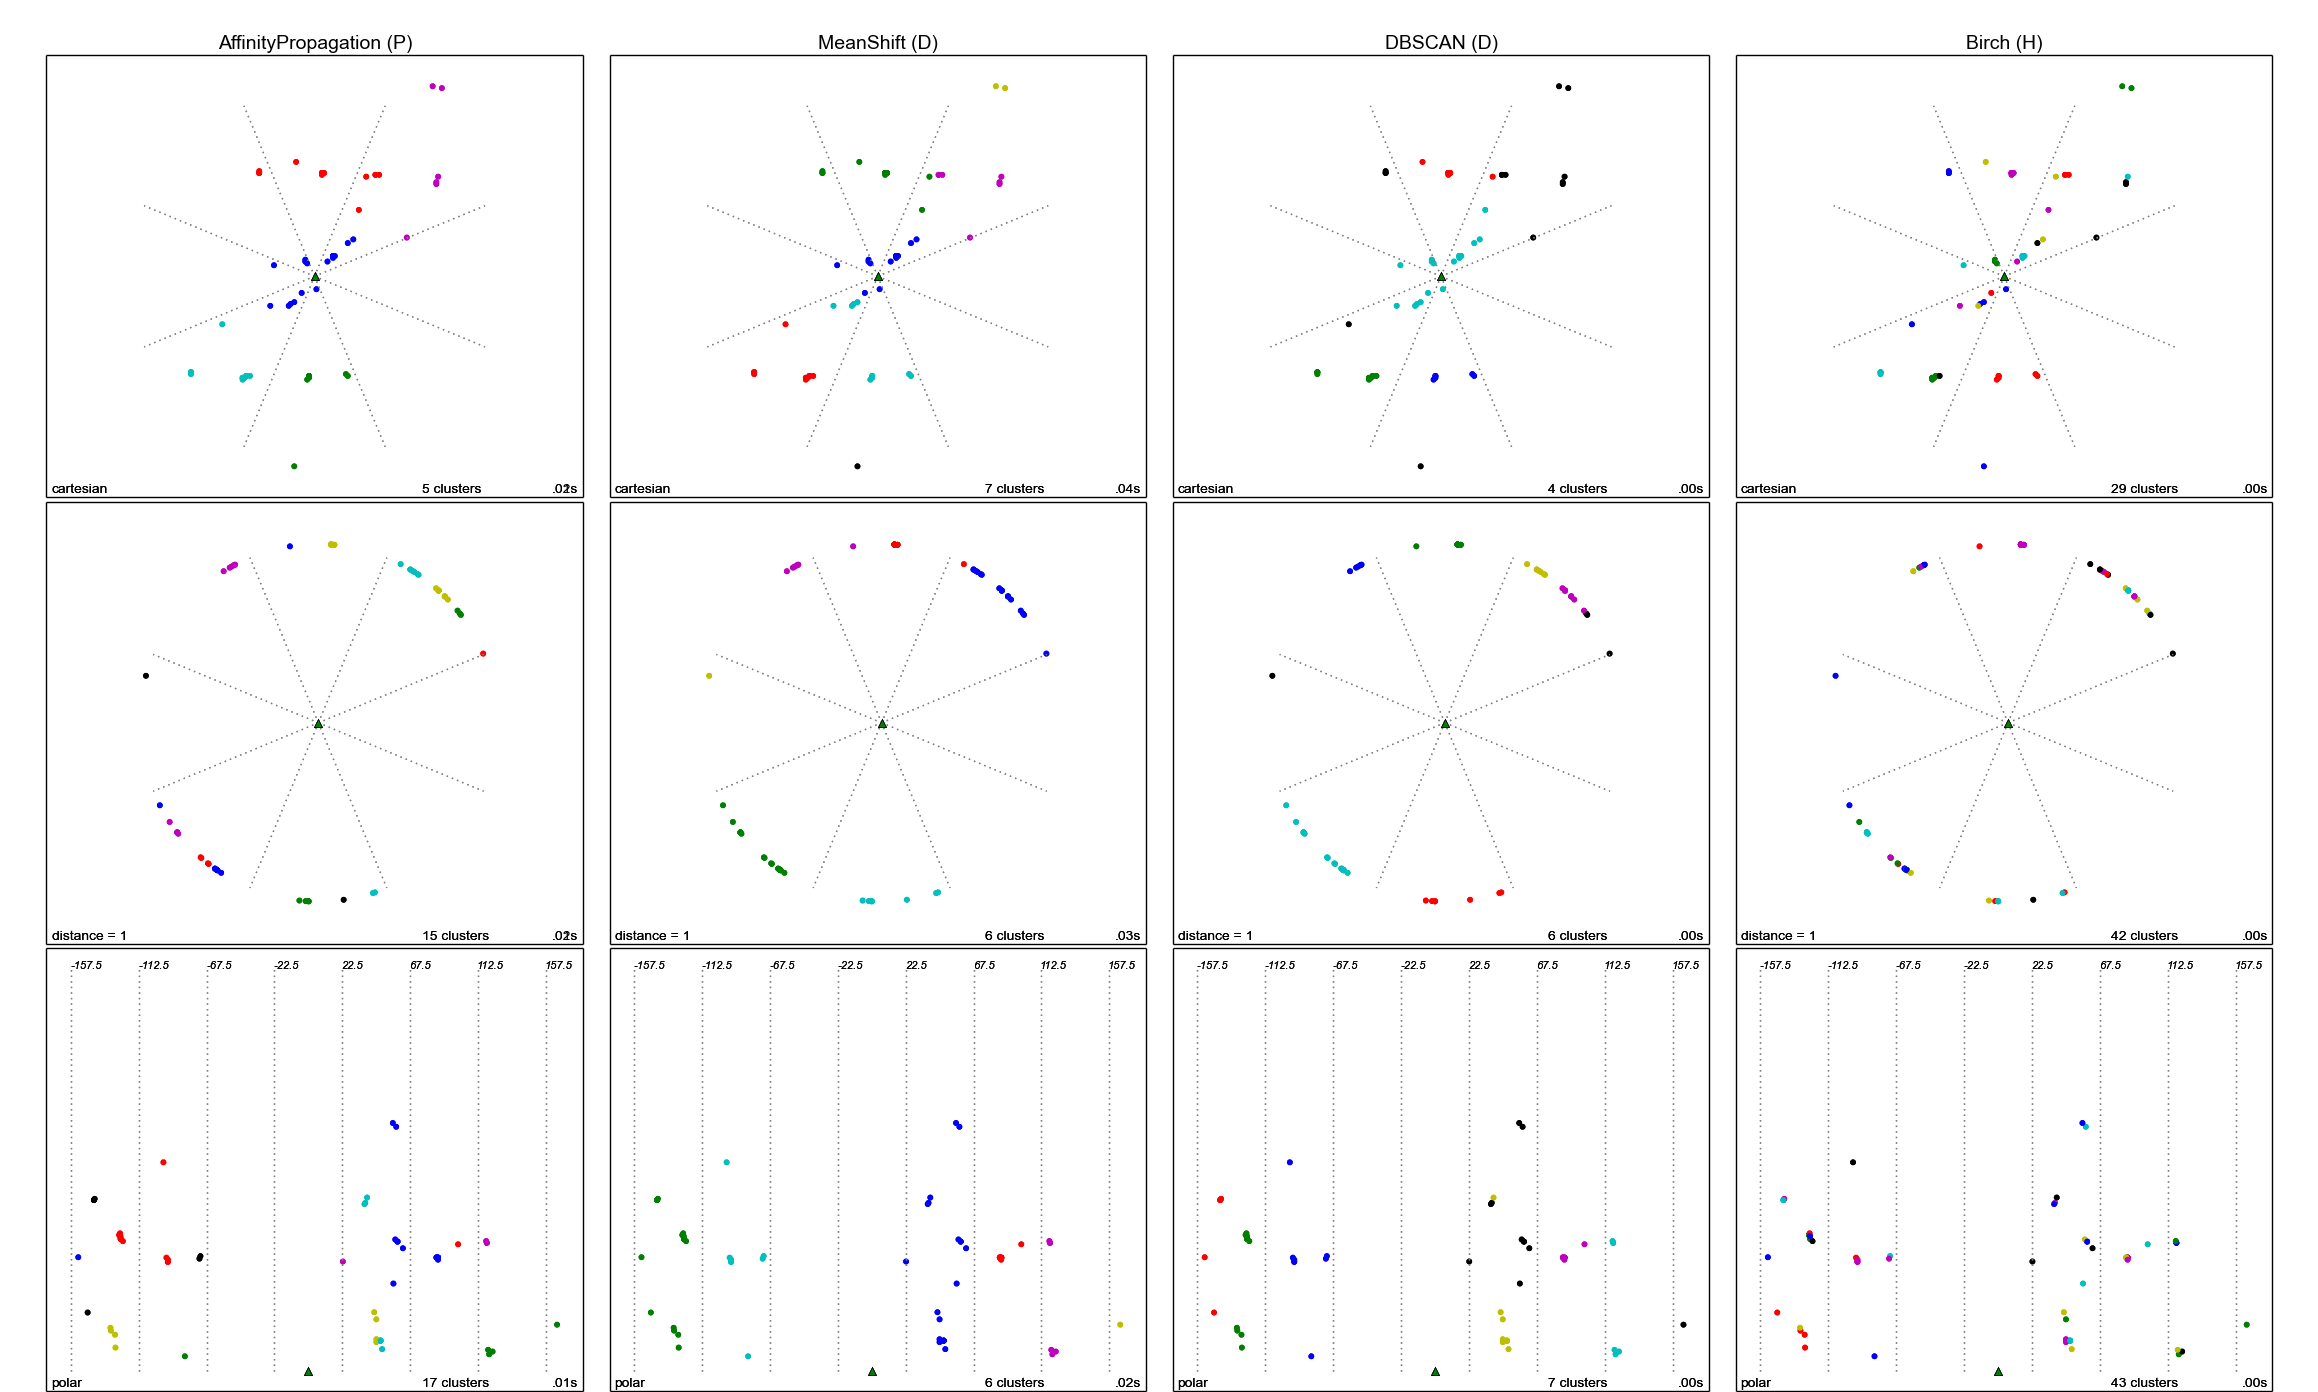
\includegraphics[width=\textwidth]{figures/comparison}
% 	\caption{Comparison between clustering algorithms. Raw data are on the first row. Below are coordinates projected in polar coordinates.}
% 	\label{fig:comparison}
% \end{figure}

% A solution found for that problem was to normalize points' distance to the origin. As a result, points are projected on a circle of radius 1. The new graph is shown in Figure~\ref{fig:comparison}. In that graph, we see that the algorithm (HDBSCAN) performs better than in the previous referential. Whereas that idea has a clear advantage in improving clustering, the concept of action' strenght is not taken into account because the focus is only done on action's direction.
%
% In extension of that normalisation, another solution was to convert coordinates from cartesian referential to polar referential. We found (give results...) that the clustering algorithms performed better with polar coordinates than with cartesian coordinates. Indeed, angular apertures are much more clearly distinguished. This is specially the case when values are separated with several close to the origin and others far from it.

\subsubsection{Implémentation}
Nous avons utilisé le framework C++ Sferes \cite{Mouret2010} développé au sein de l'équipe AMAC et dédié aux calculs évolutifs. Ce framework a pour avantages d'être léger, multi-coeur et facilement extensible. Un très grand nombre

A large amount of clustering algorithms exist and were found in a previous stage (see in Annex). Seven of them were selected (mainly partition and density-based algorithms). A problem was to find the best algorithm and parameters for a given dataset. We needed also a way to validate the parameters found.
That algorithm is used by the fitness function within the evolutionary algorithm. The proposed method consists in an iterative algorithm in which a clustering algorithm is tuned in order to satisfy three different objectives: \circled{1} the number of moves to reach the goal, to be minimized to make the robot as fast as possible, \circled{2} the number of clusters, to be minimized in order to simplify computations and \circled{3} the final distance to the goal, to be minimized for the accuracy of the control.
% As there were different objectives to minimize, we selected the NSGA-II\cite{Deb:2002:FEM:2221359.2221582} evolutionary algorithm to fulfill this task.
Dans la mesure où plusieurs objectifs sont à minimiser, nous avons sélectionné l'algorithme évolutif NSGA-II\cite{Deb:2002:FEM:2221359.2221582} pour remplir cette tâche.

\begin{algorithm}
\caption{Evaluation algorithm for fitness function}\label{euclid}
  \begin{algorithmic}[1]
    \State $E$ = \{C\textsubscript{e1}, \dots, C\textsubscript{en}\} \Comment{Set of clusters containing effects}
    \State $F$ = \{f\textsubscript{1}, \dots, f\textsubscript{n}\} \Comment{Set of final points}
    \State $I$ = (0;0) \Comment{Initial point}
    \State $t$ = 0 \Comment{Number of tries}
    \State Compute the set of effects $E$ from genotype
      \ForAll{final point $f\textsubscript{i}$ in $F$}
        \For{$j=1$ to \textit{nb\_repeat} }
          \While{$dist(I,\:f\textsubscript{i}) > \varepsilon$ \textbf{and} $t<t_{max}$}
            \State $M = \{ m\textsubscript{i}\:|\:m\textsubscript{i} = rand(C\textsubscript{ei})\:\forall\:C\textsubscript{ei}\:\in E\}$
            \State $m = \operatornamewithlimits{argmin}\limits_{m_i \in M}(dist(I+m\textsubscript{i},\:f\textsubscript{i}))$
            \State Apply movement $m$ to $I$
            \State $t = t + 1$
          \EndWhile
        \EndFor
      \EndFor
      \State return (\textoverline{nb movements}, nb clusters, \textoverline{final distance})
  \end{algorithmic}
\end{algorithm}



% \ \\In order to obtain interesting results, we realize experiments based on the following experimental design, in full factorial design :
%
% \begin{itemize}
%   \item Population size: 50, 100, 200
%   \item Number of generations: 100, 200, 500
%   \item Mutation probability: 0.1, 0.2, 0.5
%   \item Crossover rate: 0.6, 0.8, 0.7
% \end{itemize}

NSGA-II étant un algorithme multi-objectif, plusieurs meilleures solutions peuvent être trouvées, correspondants aux individus dominants le front de Pareto. La figure \ref{fig4} montre la valeur du paramètre (de l'algorithme de clustering) correspondant aux individus dominants.

\begin{figure}[ht]
  \begin{center}
  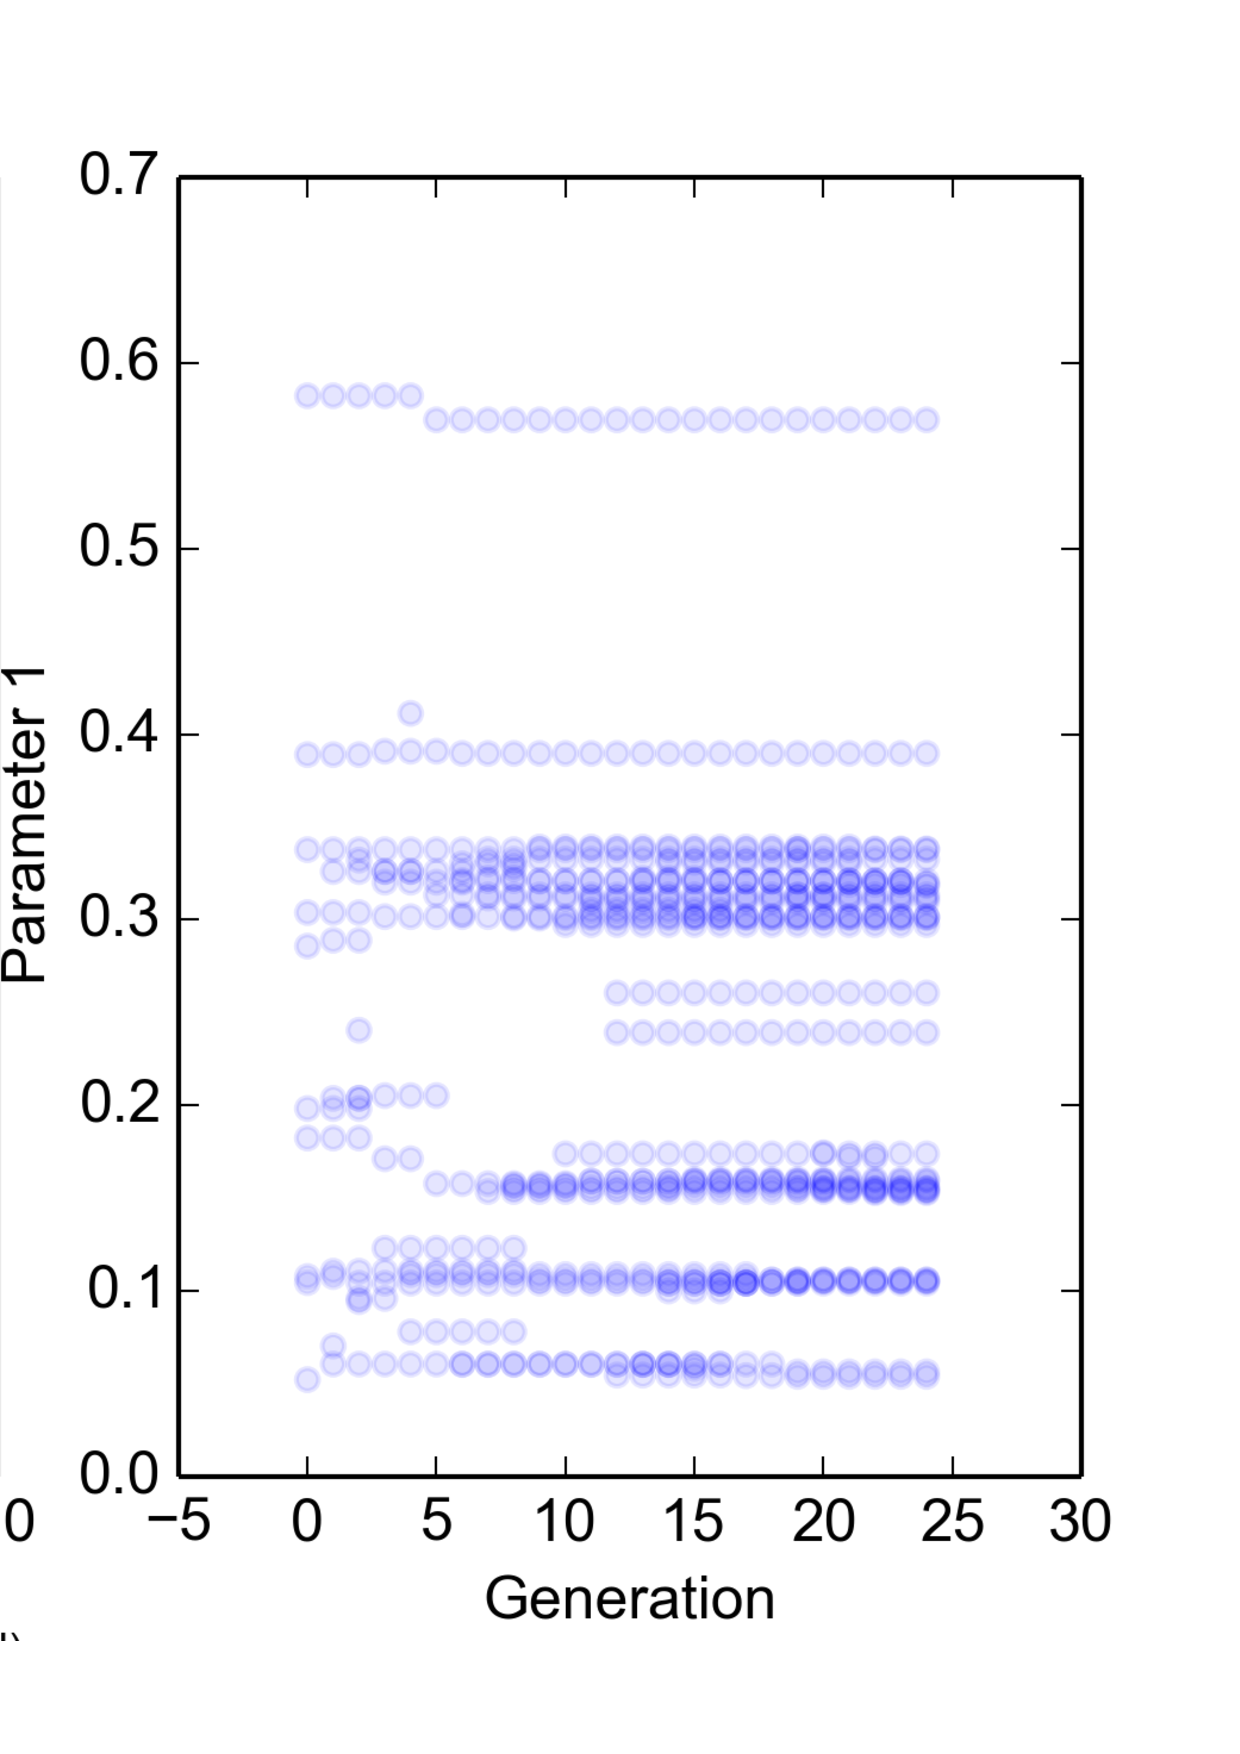
\includegraphics[width=0.4\textwidth]{figures/Pareto_front.pdf}
    \caption{Valeur du paramètre de l'algorithme de clustering Mean Shift correspondant aux individus dominants le front de Pareto.}
  \ref{fig4}
  \label{fig4}
  \end{center}
\end{figure}

\`A partir de ces meilleures valeurs de paramètres, nous avons généré (Figure \ref{fig6}) deux séries de graphiques. Les deux ensembles de clusters optimisent différents objectifs : vitesse et précision contre coût computationnel. La colonne de gauche contient davantage de clusters et permet un contrôle rapide et précis. \`A l'inverse, l'autre solution repose sur un nombre moins important de clusters.

\begin{figure}[ht]
  \begin{center}
  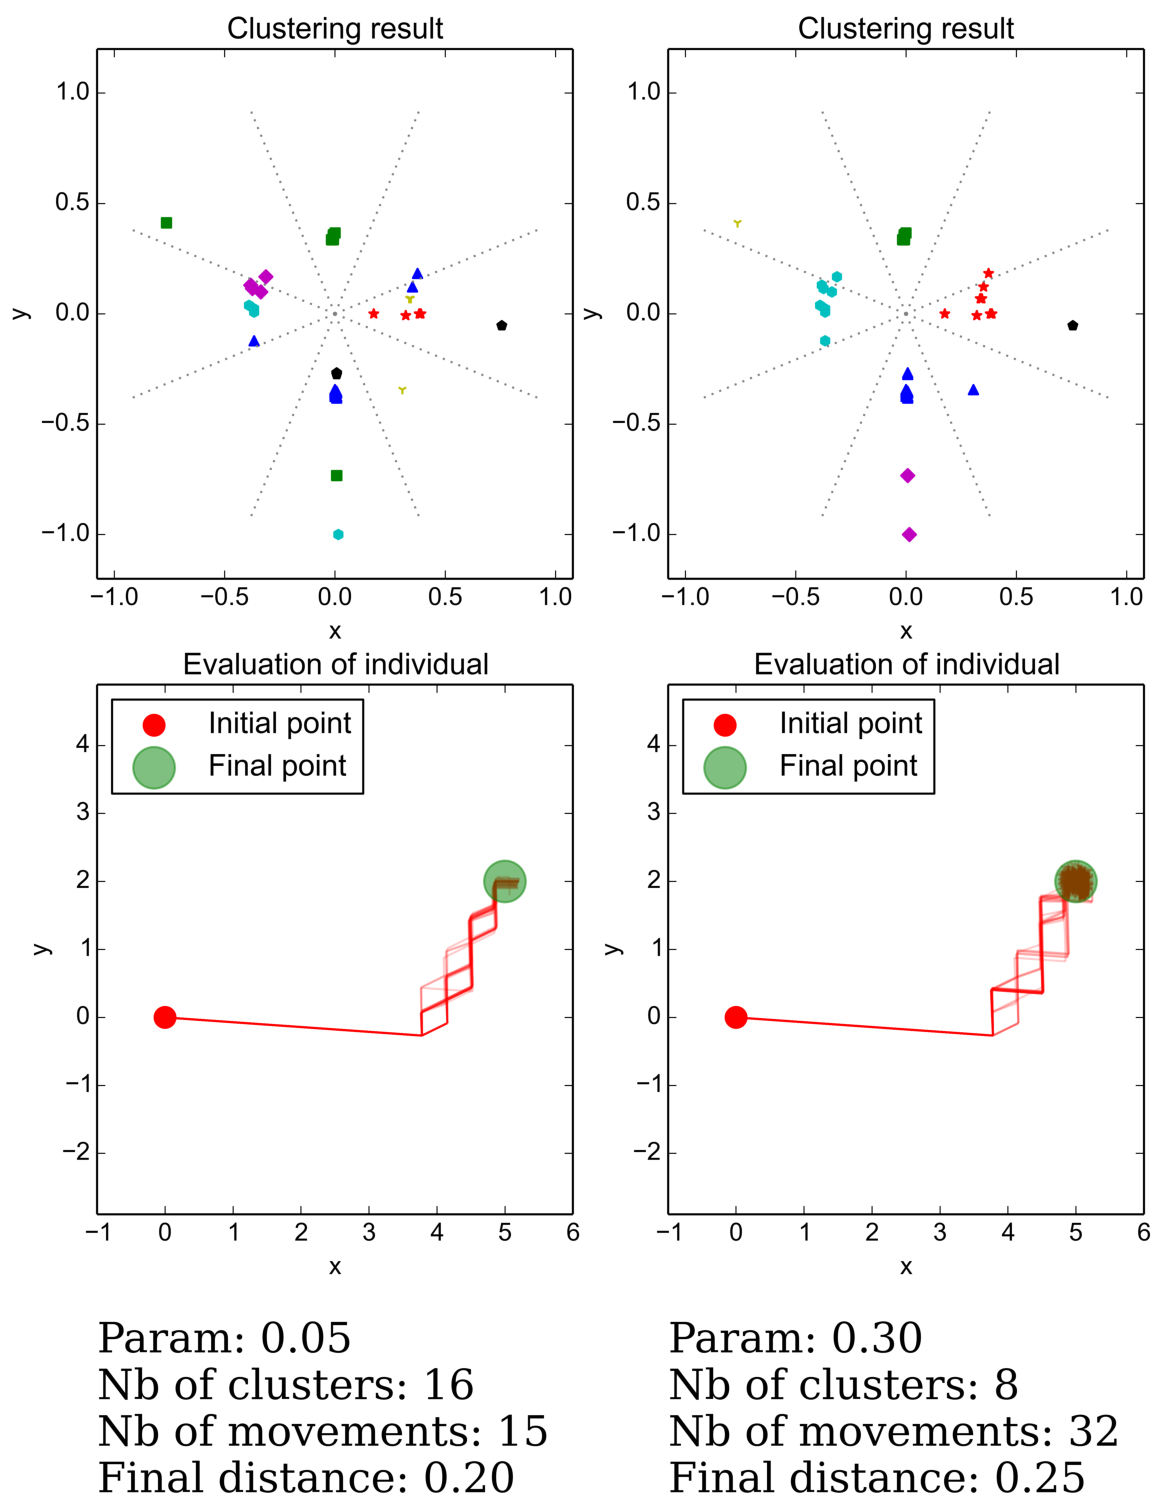
\includegraphics[width=0.5\textwidth]{figures/Benchmark_3.pdf}
  % \caption{The two columns show different clustering results and evaluation trajectories based on parameter values belonging to indivuals on Pareto Front.}
  \caption{Les deux colonnes montrent différents résultats de clustering et de trajectoires d'évaluations basés sur les valeurs de paramètres appartenant aux individus dominants le front de Pareto.}
  \label{fig6}
  \end{center}
\end{figure}

Clusterisation based on Ugur's paper: 40 features. Compare Ugur's work with us.

Cette première partie de notre stage a fait l'objet d'une soumission d'un abstract long au workshop \textit{Developmental learning and representation building in human-robots and ambient intelligence systems} de la conférence ECAL2017\footnote{https://project.inria.fr/ecal2017/} qui se tient à Lyon en septembre 2017.

% \subsection{Transfer learning on a simple task}

% \subsection{Symbolic planning}

\subsubsection{Pushing object experiment}
La seconde partie de notre stage a consisté à mener une expérience en se servant de l'algorithme de clusterisation d'effets décrit ci-dessus. Une première expérimentation a eu lieu en simulation puis à l'aide du robot réel. Cette expérience peut être divisée en 3 étapes : \circled{1} génération du babbling sensorimoteur et enregistrement des effets pour les différents objets, \circled{2} réalisation de la clusterization des effets et \circled{3} test de l'apprentissage.  Voir figure \ref{fig7} pour la mise en place initiale.

Afin d'obtenir des jeux de données contenant les différents effets à apprendre, le babillage sensorimoteur a été effectué à l'aide de l'algorithme génétique Novelty Search\cite{5949955}. Cette approche est utilisée par Maestre et al. dans \cite{Maestre2015}. Pour cela, le calcul des trajectoires est effectué dans une première étape. Pour chaque trajectoire, on regarde si elle intersecte avec le cube. Si c'est le cas, cette trajectoire est gardée et jouée par le robot en simulation. La figure \ref{fig:ns_traj} montre un exemple de trajectoire touchant l'objet considéré.


\begin{figure}[ht]
  \begin{center}
  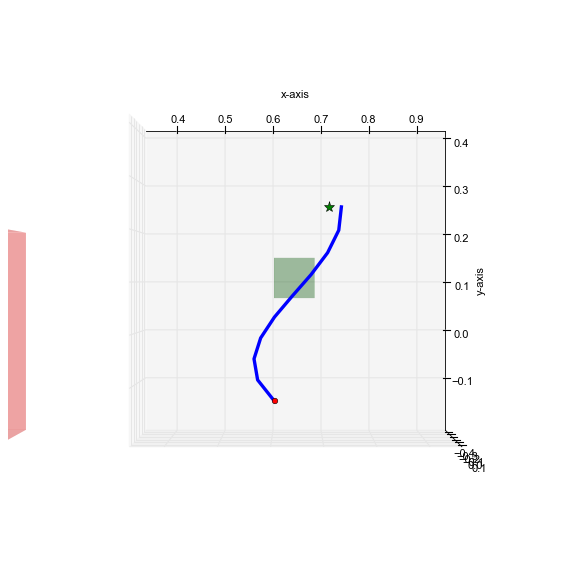
\includegraphics[width=0.7\textwidth]{figures/ns_trajectory.png}
  \caption{Le rectangle rouge indique la position du robot. Le point rouge correspond au point de départ de l'effecteur du robot. Le tracé en bleu correspond à la trajectoire de cet effecteur vers l'objet. L'étoile verte indique la position de l'objet à la fin de l'exécution de la trajectoire de l'effecteur.}
  \label{fig:ns_traj}
  \end{center}
\end{figure}

\begin{figure}[ht]
  \begin{center}
  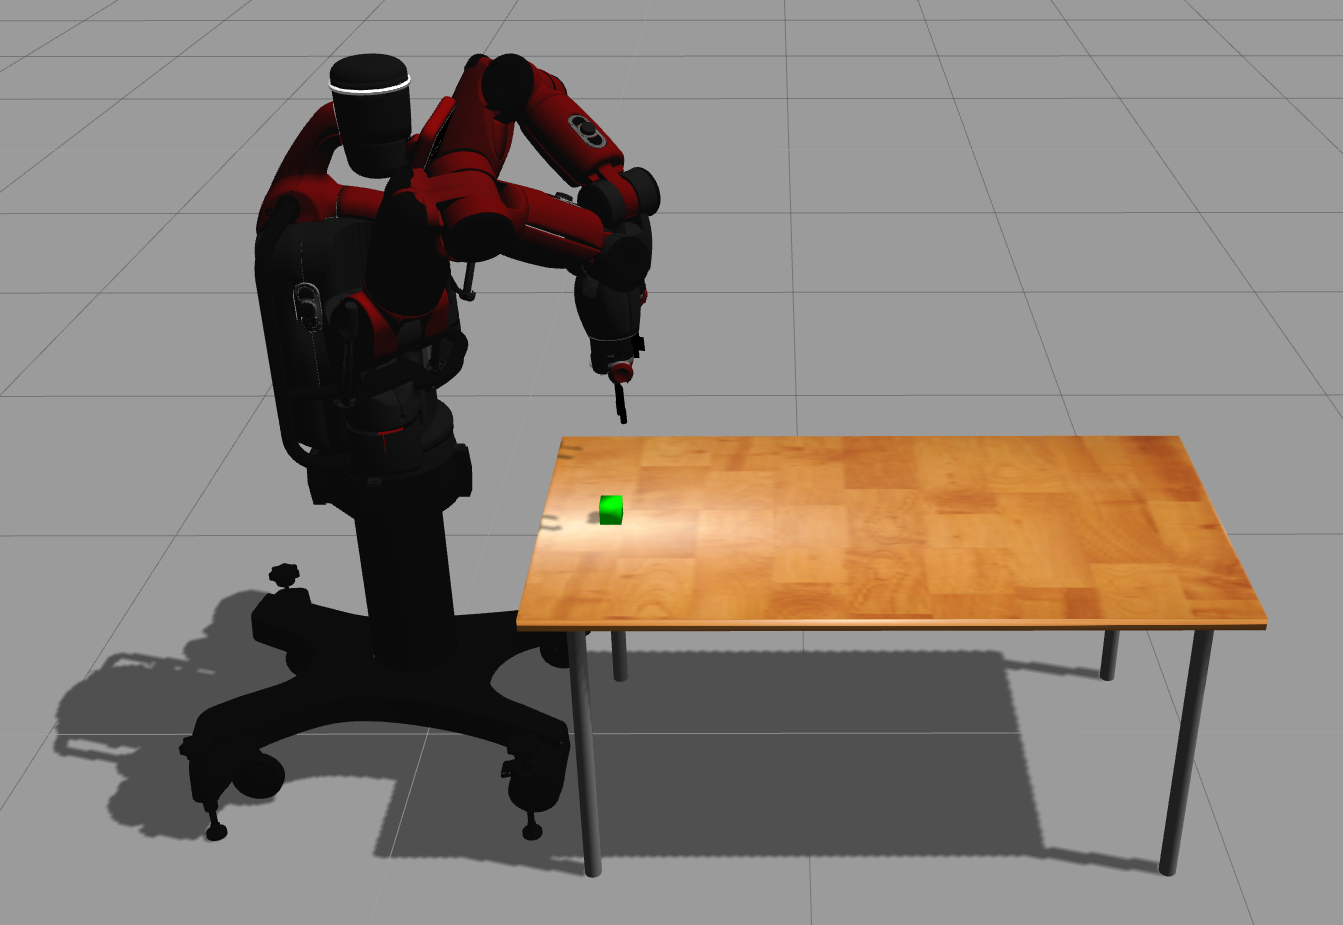
\includegraphics[width=0.7\textwidth]{figures/Experiment_setup.png}
  \caption{L'objectif du robot est d'apprendre à pousser différents objets (par exemple, un cube) depuis sa position initiale jusqu'à la zone cible.}
  \label{fig7}
  \end{center}
\end{figure}

Durant la première étape, différents objets sont placés successivement sur la table : une boîte de forme cubique, un cylindre et un cône. Ces objets ont différentes propriétés : certains peuvent être poussés à partir de n'importe quelle face et générer un comportement identique (boîte), tandis que d'autres nécessiteront d'être poussés depuis une face particulière (cylindre et cône) afin de garder une trajectoire cohérente. Le babillage réalisé par le robot sur ces différents objets permet de produire des jeux de données d'effets.
La seconde étape implique l'algorithme que nous avons présenté ci-dessus et tente de clusteriser les effets des jeux de données. Il en résulte une variété de paramètres qui peuvent être exploités durant la troisième étape.
Les meilleurs paramètres trouvés dans l'étape précédente sont utilisés pour pousser les différents objects vers la zone cible.

% During the first step, several different objects are placed on the table, one after another. Those objects have different properties: a box, a cylinder which and a cone. Some can be pushed from any face and will have the same behavior, whereas the other ones need to be pushed from a particular face to move significantly. The babbling with the different objects would result in a dataset of effects.
% The second step implies the algorithm we presented above and tries to clusterize the effects in the dataset. As result, a variety of parameter can be exploited during the third stage.
% The best parameters found in the previous stage are used for pushing the different object into the goal area.


\section{Discussion}
% \epigraph{A computer would deserve to be called intelligent if it could deceive a human into believing that it was human.}{\textit{Alan Turing}}

\section{Future works \& Perspectives}

Plusieurs axes d'améliorations peuvent être proposés. Durant ce stage, nous avons testé l'algorithme présenté ci-dessus avec un seul algorithme de clustering, \textit{Mean Shift}. Le premier axe d'amélioration consisterait à tester davantage d'algorithmes de clustering, tels qu'\textit{Affinity Propagation}, \textit{Birch} ou \textit{DBSCAN}. Un second axe d'amélioration pourrait être de tester l'algorithme avec des tâches plus complexes.

\section{Conclusion}

Ce stage de fin d'études de Master 2 m'a permis de davantage découvrir le domaine de la robotique développementale et ce qu'il implique, après la brève introduction que nous avons eu durant le semestre de M2 à Lyon. Ce domaine de recherche est fascinant et très intéressant dans la mesure où les chercheurs tendent à créer des robots qui pourraient boostrap from almost no knowledge. Le lien étroit entre neurosciences et spécialement neurosciences cognitives permet d'implémenter des modèles présent chez l'être humain.

% \section*{Annexe}
% % \addcontentsline{toc}{chapter}{Annex}
%
% % \begin{tabular}{|l|c|r|}
% %   \hline
% %   colonne 1 & colonne 2 & colonne 3 \\
% %   \hline
% %   1.1 & 1.2 & 1.3 \\
% %   2.1 & 2.2 & 2.3 \\
% %   \hline
% % \end{tabular}
%
% \begin{tabular}{ |l|l|l| }
% % \hline
% % \multicolumn{3}{ |c| }{Team sheet} \\
% \hline
% Type & Name & Since \\ \hline
% \multirow{4}{*}{Partitionnement} & LB & Lucas Radebe \\
%  & DC & Michael Duburry \\
%  & DC & Dominic Matteo \\
%  & RB & Didier Domi \\ \hline
% \multirow{3}{*}{Basé sur la densité} & MC & David Batty \\
%  & MC & Eirik Bakke \\
%  & MC & Jody Morris \\ \hline
% \multirow{2}{*}{Grid based} & ST & Alan Smith \\
%  & ST & Mark Viduka \\
% \hline
% \end{tabular}

\bibliographystyle{unsrt}
\bibliography{./LEROY_M2_ISIR_2017_internship_thesis.bib}

\end{document}
